% Options for packages loaded elsewhere
\PassOptionsToPackage{unicode}{hyperref}
\PassOptionsToPackage{hyphens}{url}
%
\documentclass[12pt]{article}
\usepackage{amsmath,amssymb}
\usepackage{lmodern}
\usepackage{iftex}
\ifPDFTeX
  \usepackage[T1]{fontenc}
  \usepackage[utf8]{inputenc}
  \usepackage{textcomp} % provide euro and other symbols
\else % if luatex or xetex
  \usepackage{unicode-math}
  \defaultfontfeatures{Scale=MatchLowercase}
  \defaultfontfeatures[\rmfamily]{Ligatures=TeX,Scale=1}
\fi
% Use upquote if available, for straight quotes in verbatim environments
\IfFileExists{upquote.sty}{\usepackage{upquote}}{}
\IfFileExists{microtype.sty}{% use microtype if available
  \usepackage[]{microtype}
  \UseMicrotypeSet[protrusion]{basicmath} % disable protrusion for tt fonts
}{}
\makeatletter
\@ifundefined{KOMAClassName}{% if non-KOMA class
  \IfFileExists{parskip.sty}{%
    \usepackage{parskip}
  }{% else
    \setlength{\parindent}{0pt}
    \setlength{\parskip}{6pt plus 2pt minus 1pt}}
}{% if KOMA class
  \KOMAoptions{parskip=half}}
\makeatother
\usepackage{xcolor}
\usepackage{longtable,booktabs,array}
\usepackage{calc} % for calculating minipage widths
% Correct order of tables after \paragraph or \subparagraph
\usepackage{etoolbox}
\makeatletter
\patchcmd\longtable{\par}{\if@noskipsec\mbox{}\fi\par}{}{}
\makeatother
% Allow footnotes in longtable head/foot
\IfFileExists{footnotehyper.sty}{\usepackage{footnotehyper}}{\usepackage{footnote}}
\makesavenoteenv{longtable}
\usepackage{graphicx}
\makeatletter
\def\maxwidth{\ifdim\Gin@nat@width>\linewidth\linewidth\else\Gin@nat@width\fi}
\def\maxheight{\ifdim\Gin@nat@height>\textheight\textheight\else\Gin@nat@height\fi}
\makeatother
% Scale images if necessary, so that they will not overflow the page
% margins by default, and it is still possible to overwrite the defaults
% using explicit options in \includegraphics[width, height, ...]{}
\setkeys{Gin}{width=\maxwidth,height=\maxheight,keepaspectratio}
% Set default figure placement to htbp
\makeatletter
\def\fps@figure{htbp}
\makeatother
\setlength{\emergencystretch}{3em} % prevent overfull lines
\providecommand{\tightlist}{%
  \setlength{\itemsep}{0pt}\setlength{\parskip}{0pt}}
\setcounter{secnumdepth}{-\maxdimen} % remove section numbering
\ifLuaTeX
  \usepackage{selnolig}  % disable illegal ligatures
\fi
\IfFileExists{bookmark.sty}{\usepackage{bookmark}}{\usepackage{hyperref}}
\IfFileExists{xurl.sty}{\usepackage{xurl}}{} % add URL line breaks if available
\urlstyle{same} % disable monospaced font for URLs
\hypersetup{
  hidelinks,
  pdfcreator={LaTeX via pandoc}}

\author{}
\date{}

\usepackage{imakeidx}
\makeindex
\usepackage[margin=1.5cm]{geometry}
\usepackage{graphicx,subcaption,lipsum}
\bibliographystyle{ieeetr}
\usepackage{biblatex}
\bibliography{references}

\begin{document}
\begin{center}

\includegraphics[width = 0.4\textwidth]{Picture 1.jpg}
\section{B-Tech Project Sep-Dec 2023}
\hfill \break
\hfill \break
\end{center}
\begin{center}
\large{\textbf{TESTING THE STATISTICAL ISOTROPY OF GAMMA RAY BURSTS' SKY DISTRIBUTION}}
\end{center}

\hfill \break
\begin{center}
\hfill \break
\hfill \break
\textbf{ASHWIN GANESH}
\\
\textbf{EP21BTECH11009}
\\
\hfill \break
\hfill \break
\textbf{Under the guidance of}
\\
\large{\textbf{Dr. Shantanu Desai}}
\\
\hfill \break
\hfill \break
\textbf{DEPARTMENT OF PHYSICS}
\\
\textbf{INDIAN INSTITUTE OF TECHNOLOGY HYDERABAD}
\end{center}
\clearpage


\hfill \break
\hfill \break
\hfill \break
\hfill \break
\hfill \break
\hfill \break
\hfill \break
\begin{center}
    \section{DECLARATION}
{\large I declare that this written submission represents my ideas in my own
words, and where ideas or words of others have been included, I have adequately
cited and referenced the original sources. I also declare that I have
adhered to all principles of academic honesty and integrity and not have
misrepresented or fabricated or falsified any idea/data/fact/source in
my submission. I understand that any violation of the above will be a
cause for disciplinary action by the Institute and can also evoke penal
action from the sources that have thus not been properly cited, or from
whom proper permission has not been taken when needed.}
\end{center}

\clearpage

\hfill \break
\hfill \break
\hfill \break
\hfill \break
\hfill \break
\hfill \break
\hfill \break
\begin{center}
    \section{ACKNOWLEDGEMENTS
}
{\large I sincerely thank Dr. Shantanu Desai for his constant guidance and
support. I have gained valuable knowledge and some much-needed clarity about my future from this project, and I can't thank him enough.}
\end{center}
\newpage


\hfill \break
\hfill \break
\hfill \break
\hfill \break
\hfill \break
\hfill \break
\hfill \break
\begin{center}
    \section{APPROVAL SHEET}

{\large This report titled ``TESTING THE STATISTICAL ISOTROPY OF GAMMA RAY
BURSTS' SKY DISTRIBUTION'' is submitted by Ashwin Ganesh as a part of his BTech Project.}
\end{center}
\newpage


\hfill \break
\hfill \break
\hfill \break
\hfill \break
\hfill \break
\hfill \break
\hfill \break
\section{ABSTRACT}


One of the main hypotheses of standard cosmology is the assumption of
homogeneity and isotropy. In this study, we explore and test this
hypothesis using the two-point angular correlation function of numerous
gamma-ray bursts (GRB) from BATSE, SWIFT and FERMI GRB catalogues. We
show that the uncertainties in the position of the GRBs induces
anisotropy in the sky distribution. However, even after these
uncertainties are taken into account, it is found that the anisotropy
still persists in some cases. This result is in contrary to numerous
other reports which prove that the assumption of isotropy holds true.\cite{andrade2019revisiting}

\textbf{Key words : Large-scale structure of Universe – methods: data analysis – gamma-ray burst: general}
\newpage
{\Large\textbf{CONTENT}}

\begin{enumerate}
\def\labelenumi{\arabic{enumi}.}
\item
  Introduction\index{Introduction}

  \begin{enumerate}
  \def\labelenumii{\arabic{enumii}.}
  \item
    Cosmological Principle.................................................................................................................(7)
  \item
    Gamma Ray Bursts......................................................................................................................(7)
  \item
    Observational Data Set................................................................................................................(8)
  \end{enumerate}
\item
  Data Analysis

  \begin{enumerate}
  \def\labelenumii{\arabic{enumii}.}
  \item
    Two-point angular correlation function.......................................................................................(9)
  \item
    Absolute sum test.......................................................................................................................(9)
  \item
    Statistical significance estimate..................................................................................................(10)
  \item
    GRB positional uncertainties.....................................................................................................(10)
  \end{enumerate}
\item
  Plots, Figures and Tables

  \begin{enumerate}
  \def\labelenumii{\arabic{enumii}.}
  \item Positional Uncertainty Histogram..............................................................................................(12)
  \item
    Absolute Sum Test.....................................................................................................................(13)
  \item
    2pACF Graphs..........................................................................................................................(16)
  \item
    KS and AD Test Results............................................................................................................(19)
\item 
3D PLOTS OF DATASETS.......................................................................................................(20)
  \end{enumerate}
\item
Results and Discussion......................................................................................................................(23)
\item 
Bibliography.....................................................................................................................................(24)
\end{enumerate}
\newpage
{\huge CHAPTER 1}

\section{\textbf{INTRODUCTION}}
\hfill \break

\textbf{\begin{enumerate}
\def\labelenumi{\arabic{enumi}.}
\item
  COSMOLOGICAL PRINCIPLE
\end{enumerate}}

The cosmological principle (CP) is one of the foundations of modern
cosmology. The cosmological principle is the notion that on a large
scale, the universe is both homogeneous and isotropic. When viewed on a
large enough scale, the forces are expected to act equally throughout
the universes on a large scale, and should, therefore, produce no
observable inequalities in the large-scale structuring over the course
of evolution of the matter field that the Big Bang initially laid down.
The cosmological principle is the second pillar of the Big Bang Model.
Recent statistical analyses on cosmological observations bring evidence
that the CP holds true, as obtained from the Cosmic Microwave Back-
ground (CMB) temperature anisotropies \cite{refId0}, cosmic
distances from type 1a Supernovae \cite{PhysRevD.97.083518} etc. 
However, some controversial claims have also appeared in literature, such as large-angle features in the CMB \cite{schwarz2016cmb} and a large dipole anisotropy in radio source counts \cite{singal2011large}.
\\
\newline

\textbf{\begin{enumerate}
\def\labelenumi{\arabic{enumi}.}
\setcounter{enumi}{1}
\item
  GAMMA RAY BURSTS
\end{enumerate}
}
Gamma-ray bursts (GRBs) are the most powerful and violent explosions in
the known universe. The intense radiation of most observed GRBs is
thought to be released during a supernova or super luminous supernova as
a high-mass star implodes to form a neutron star or a black hole. Some
even originate from the merger of binary neutron stars. They reveal
themselves as possible formidable distance indicators. Gamma-ray bursts have also been used to test CP. They are usually classified into long-lived (T­\textsubscript{90} \textgreater{} 2s,
LGRBs) and short-lived \\(T\textsubscript{90} \textless{} 2s, SGRBs),
where T\textsubscript{90} denotes the time over which a burst emits from
5\% of its total measured count to 95\%.

Given the relevance of the topic, and the current controversies, we
revisit in this paper the question of the statistical isotropy in the
GRB sky distribution. The analysis performed uses the two-point angular
correlation function (2pACF) of numerous gamma-ray bursts of the FERMI \cite{von2020fourth} \cite{gruber2014fermi},
SWIFT \cite{SWIFT} and BATSE gamma-ray burst catalogue (NASA HEASARC).
\newline
\newpage
\begin{enumerate}
\def\labelenumi{\Roman{enumi}.}
\item
  FERMI GRB CATALOGUE:
  \begin{quote}
      The FERMI GBM (Gamma-ray Burst Monitor) has been operational since 2008, and includes two sets of detectors: twelve sodium iodide (NaI) scintillators, each 12.7 cm in diameter by 1.27 cm thick, and two cylindrical bismuth germanate (BGO) scintillators, each 12.7 cm in diameter and 12.7 cm in height. The NaI detectors are sensitive in the lower end of the energy range, from a few keV to about 1 MeV and provide burst triggers and locations. The BGO detectors cover the energy range ~150 keV to ~30 MeV, providing a good overlap with the NaI at the lower end and with the LAT (Large Area Telescope) at the high end.
      The earliest and latest GRB in our FERMI dataset was detected on 14 July, 2008 and on 11th September 2023 respectively. Overall, we use 3016 LGRBs and 596 SGRBs from this dataset.
  \end{quote}
  \hfill\break
\item
SWIFT GRB CATALOGUE:
\begin{quote}
    SWIFT is a first-of-its-kind multi-wavelength observatory dedicated to the study of gamma-ray burst (GRB) science. Operational since 2004, its three instruments work together to observe GRBs and afterglows in the gamma-ray, X-ray, ultraviolet, and optical wavebands. The Burst Alert Telescope (BAT) is sensitive in the energy range between 15 - 150 keV. The X-ray Telescope (XRT) operates in the energy range of 0.3 - 10 keV. The UV/Optical Telescope (UVOT) takes images and can obtain spectra (via a grism filter) of GRB afterglows during pointed follow-up observations. 
    The earliest and latest GRB in our SWIFT dataset was detected on 17th January, 2005 and 26th August 2023 respectively. Overall, we use 1151 LGRBs and 92 SGRBs from this dataset.
\end{quote}
\hfill \break
\item 
BATSE GRB CATALOGUE:
\begin{quote}
    BATSE was a high energy astrophysics experiment in orbit around Earth on NASA's Compton Gamma-Ray Observatory. It was operational from 1991 to 2000. It carried a complement of four instruments that covered an unprecedented six orders of the electromagnetic spectrum, from 20 keV to 30 GeV. The earliest and latest GRB in our BATSE dataset was detected on 21st April, 1991 and 26th May 2000 respectively. Overall, we use 1299 LGRBs and 236 SGRBs from this dataset.
\end{quote}
\end{enumerate}
\newpage
\textbf{\begin{enumerate}
\def\labelenumi{\arabic{enumi}.}
\setcounter{enumi}{2}
\item
  OBSERVATIONAL DATA SET
\end{enumerate}}

As mentioned earlier, we will be using the Fermi, Batse and Swift
databases. Specifically, we use these four quantities in our analysis:

\begin{enumerate}
\def\labelenumi{\Roman{enumi}.}
\item
  RA : The Right Ascension of the burst, given in J2000 decimal degree
  \begin{quote}
      Right Ascension is the celestial equivalent of longitude. It is the angular distance of a body's hour circle east of the vernal equinox, measured along the celestial equator (east -- west coordinate). RA can be expressed in degrees, but it is more common to specify it in hours, minutes, and seconds of time: the sky appears to turn 360° in 24 hours, or 15° in one hour. So an hour of RA equals 15° of sky rotation.
  \end{quote}
\item
  DEC : The Declination of the burst, given in J2000 decimal degree
  \begin{quote}
The Declination is the celestial equivalent of latitude. For DEC, + and
- refer to north and south, respectively. The celestial equator is 0°
DEC, and the poles are +90° and -90°.
\end{quote}
\end{enumerate}

\begin{enumerate}
\def\labelenumi{\Roman{enumi}.}
\setcounter{enumi}{2}
\item
  Error radius : The uncertainty of the object position in degrees. 
  \begin{quote}
  We term it as \(\sigma\)\textsubscript{r}, which ranges from zero, up to
  \textasciitilde68°
\end{quote}
\item
  T­\textsubscript{90} : The duration, in seconds, during which 90\% of the burst fluence was accumulated.
\end{enumerate}

We test the statistical isotropy for the LGRB and SGRB sub-samples of the three datasets.
\newpage

{\huge CHAPTER 2}

\section{\textbf{DATA ANALYSIS}}

\textbf{\begin{enumerate}
\def\labelenumi{\arabic{enumi}.}
\item
  TWO-POINT AUTOCORRELATION FUNCTION
\end{enumerate}}

One can report the mean number of points at a specific scale to describe
the distribution of data points in the sky. Nevertheless, because this
measure is not sensitive to grouping, the mean might not be a good enough descriptor in the presence of clustering. The 2pACF statistic, represented by 
\(\omega\)\((\theta),\) can be used to characterize how objects cluster in the sky. We can determine the 2pACF from the data using the well-known Landy-Szalay estimator \cite{landy1993bias},

\begin{center}
    \(\omega\)\((\theta)\) = \(\dfrac{\langle DD(\theta)\rangle - 2\langle DR(\theta)\rangle\ + \langle RR(\theta)\rangle}{\langle RR(\theta)\rangle}\)
\end{center}


where the brackets denote the normalised number of all GRB pairs in the real data (DD(\(\theta\))), in the auxiliary random isotropic catalogue (RR(\(\theta\))), and between the data and the random catalogue (DR(\(\theta\))). The counts of pairs for each angular scale is carried out through the range \((\theta-d\theta/2, \theta+d\theta/2)\), where \(d\theta\) is the bin width
Essentially, it provides the probability to find a pair of object
encompassed in a given solid angle with respect to an isotropic
distribution. A null value suggests the absence of clustering and it is
statistically similar for all angular scales if the underlying
distribution is isotropic.

We determine the 2pACF from the data using the
bootstrap\_two\_point\_angular function from the astroML module.
We choose evenly spaced samples in our analysis so that \(\omega\)\((\theta),\) is calculated over the interval (0°, 180°) with d\(\theta\) = 1.8°. The random
isotropic catalogues are generated following a random distribution on a
sphere.

We use the boot-strap method \cite{10.1093/mnras/stx2356} to assess our uncertainties of the 2pACF.
We derive a bootstrap sampling distribution of the 2pACF, whose
uncertainty is the sampling distribution\textquotesingle s standard
deviation, using 100 resampling between the data and the random
catalogue. We also perform the bootstrap analysis on the isotropic
random sample and compute the 2pACF using the Monte Carlo (MC) method.
Since this distribution\textquotesingle s mean and standard deviation
offer the 2pACF limitations that a finite isotropic sample needs to
meet, we refer to them as the benchmark. A notable divergence from this
standard would suggest deviations from statistical isotropy.

\textbf{\begin{enumerate}
\def\labelenumi{\arabic{enumi}.}
\setcounter{enumi}{1}
\item
  ABSOLUTE SUM TEST
\end{enumerate}}
We use the ``absolute sum test'' to look at the anisotropic signal's
readability in more detail. We define it as the sum of the absolute
values of the 2pACF function within a specific angular scale, i.e.,
\begin{center}
    \(Absolute Sum \equiv \sum_{i}|\omega(\theta)|_i\; \forall i \in\Delta\theta\),
\end{center}

where \(\Delta\theta\) is the angular range at which we split the \(\omega\)\((\theta),\) so that we perform this summation in a tomographic fashion. We choose \(\Delta\theta\) = 20° in order to have at least 10 values of \(\omega\)\((\theta),\) in an interval (since \(\Delta\theta\) = 1.8°) and thus a robust statistic for each i-bin.

Hence we can compare the 2pACF at different angular scales for the two
distributions, the real data set versus the benchmark. Again, any
significant deviation besides the error bars suggests potential
deviation from statistical isotropy.
\newpage
\textbf{\begin{enumerate}
\def\labelenumi{\arabic{enumi}.}
\setcounter{enumi}{2}
\item
  STATISTICAL SIGNIFICANCE ESTIMATE
\end{enumerate}
}
We assess the statistical significance of our analysis by means of
non-parametric tests between two different samples as follows:

\begin{enumerate}
\def\labelenumi{\Roman{enumi}.}
\item
  Kolmogorov-Smirnov (KS)
\end{enumerate}
\begin{quote}
    The Kolmogorov--Smirnov test is a nonparametric goodness-of-fit test and
is used to determine whether two distributions differ, or whether an
underlying probability distribution differs from a hypothesized
distribution. \cite{ivezic2020statistics} It is used when we have two samples coming from two
populations that can be different.
This test relies on a metric which measures the maximum distance of the
two empirical cumulative distributive function (ECDF) Fm(x) and Gn(x),
\begin{center}
\(D = max|F_m(x)-G_m(x)|\)
\end{center}

We use the function ks\_2samp from the submodule scipy.stats to carry
out this test.

\end{quote}



\begin{enumerate}
\def\labelenumi{\Roman{enumi}.}
\setcounter{enumi}{1}
\item
  Anderson-Darling (AD)
\end{enumerate}

\begin{quote}
    The Anderson-Darling test is used to test if a sample of data came from
a population with a specific distribution. \cite{scholz1987k} It is a modification of the
Kolmogorov-Smirnov (K-S) test and gives more weight to the tails than
does the K-S test. This test is based on the following statistics
\begin{center}
    \(A^2_mn = \frac{mn}{N} \int\limits_{-\infty}^\infty \frac{\{F_m(x) - G_n(x)\}^2}{H_N(x)\{1-H_N(x)\}}dH_n(x)\)
\end{center}

Fm and Gn are ECDF for two independent samples that may have different
number of points, namely n and m, respectively.
We use the function anderson\_ksamp from the submodule scipy.stats to
carry out this test.
\end{quote}


Our null hypothesis is that the two samples are drawn from the same
distribution. As mentioned earlier, the AD test is more sensitive to the
tail differences while the KS test is sensitive to the localisation, the
scale and the differences near the centre of the distribution. In this
sense, the two parametric tests are complementary.

We choose \(\alpha\) = 0.05 as the significance level at which we reject our null
hypothesis. Meaning, a p-value less than 0.05 suggests that the samples
are not drawn from the same distribution and thus denote departure from
statistical isotropy.
\hfill\break
\textbf{\begin{enumerate}
\def\labelenumi{\arabic{enumi}.}
\setcounter{enumi}{3}
\item
  GRB POSITIONAL UNCERTAINTIES
\end{enumerate}
}

Previous works have shown that the uncertainty in position might affect
the calculation of the 2pACF of their celestial distribution \cite{Tegmark_1996}. In order
to nullify the impact of such uncertainties in our study, we produce 100
Monte Carlo realisations with the following prescription,

\begin{center}
    \(RA_{new} = \mathcal{N}(RA,\sigma_r^2)\)\\
    \(DEC_{new} = \mathcal{N}(DEC,\sigma_r^2)\)\\
\end{center}

As the GRB celestial positions are getting shuffled, we call this test
MC-shuffle. We compute the 2pACF for each of these realisations,
calculate the overall mean and standard deviation and compare it with
the benchmark. We do this procedure with an uncertainty cut-off of 6°
\begin{center}
    \(\sigma_r\leq6\)°
\end{center}
\newpage



{\huge CHAPTER 3}

\section{\textbf{PLOTS, FIGURES \& TABLES}}

\textbf{\begin{enumerate}
\def\labelenumi{\arabic{enumi}.}
\item 
POSITIONAL UNCERTAINTY HISTOGRAM
\end{enumerate}
}
The following plots are to give a rough idea of how the error radius of the GRBs in each of the datasets look like. It also gives a good idea of how many GRBs we are losing because of the uncertainty cutoff.
\begin{figure}
    \centering
    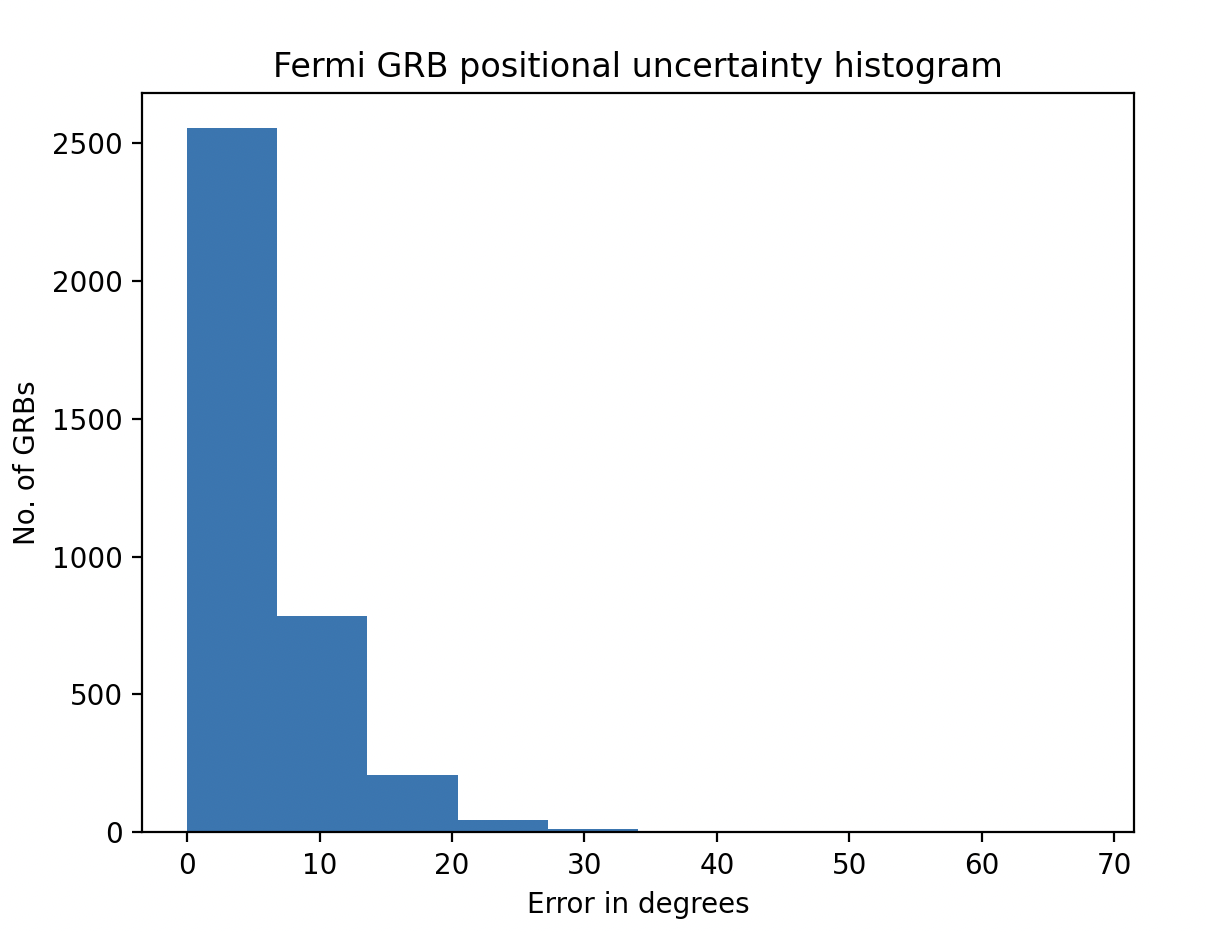
\includegraphics[width=0.5\textwidth]{Fermi GRB positional uncertainties.png}
    \caption{Histogram of the positional uncertainty of the FERMI dataset.}
    \label{fig:enter-label}
\end{figure}
\begin{figure}
    \centering
    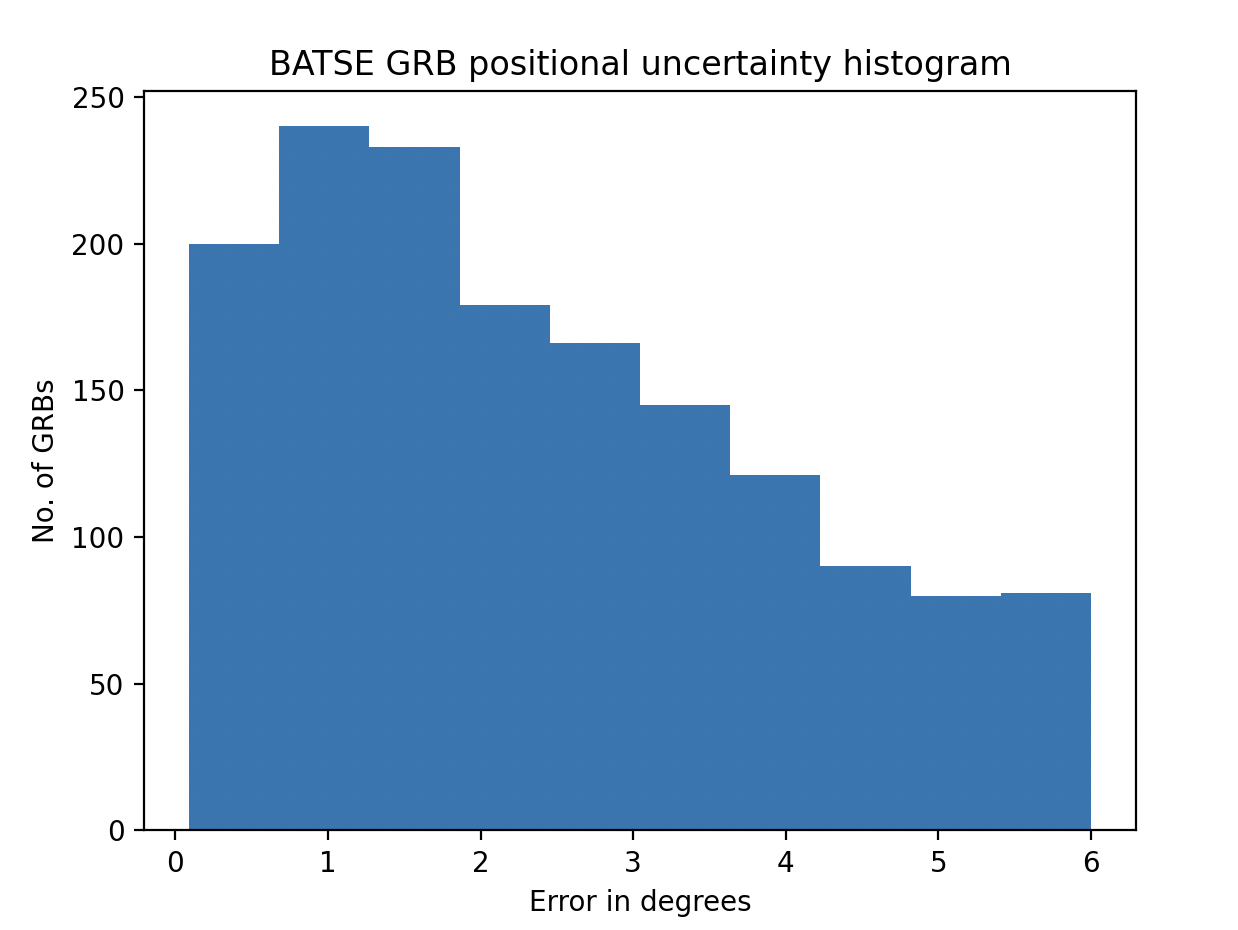
\includegraphics[width=0.5\textwidth]{BATSE GRB positional uncertainty.png}
    \caption{Histogram of the positional uncertainty of the BATSE dataset.}
    \label{fig:enter-label}
\end{figure}
\begin{figure}
    \centering
    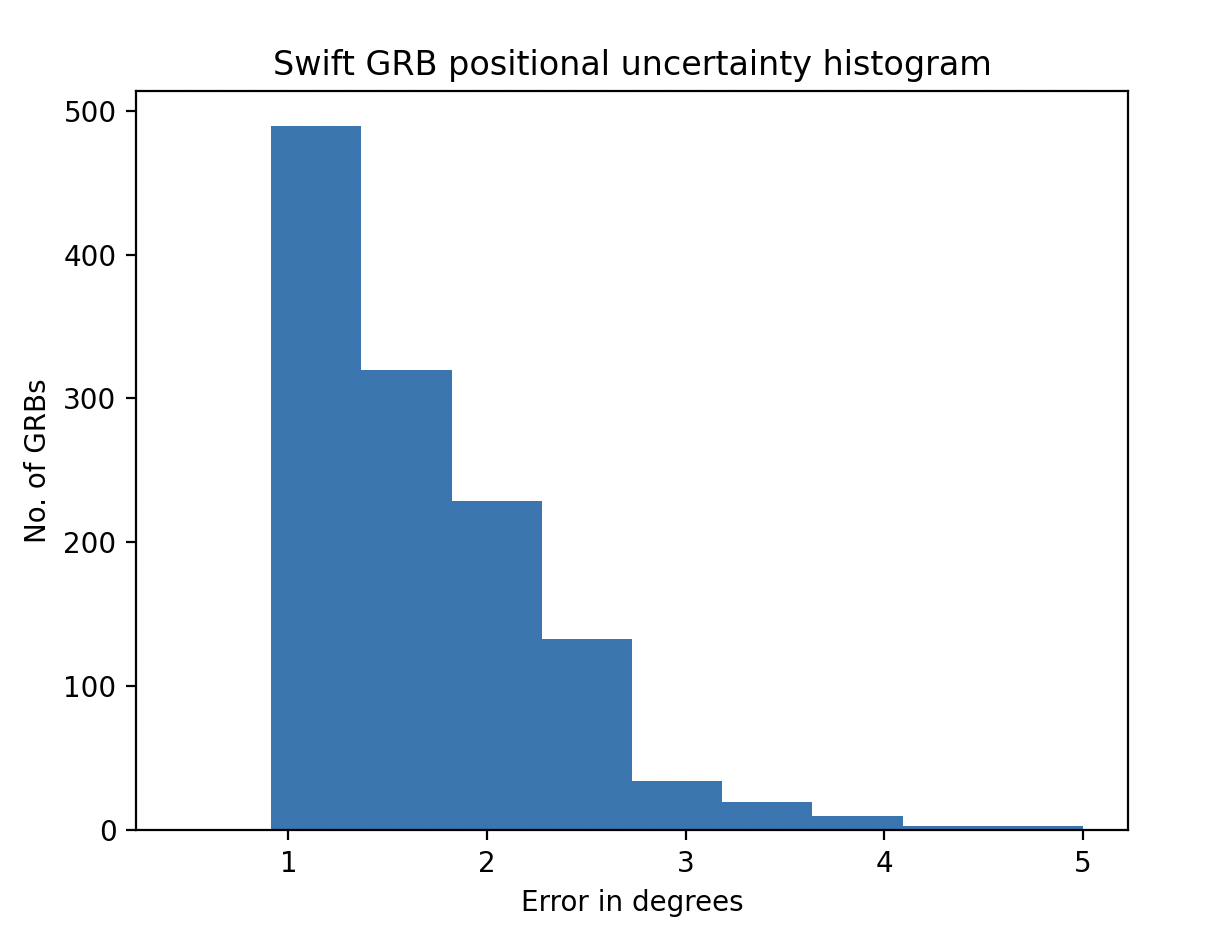
\includegraphics[width=0.5\textwidth]{Swift Histogram.png}
    \caption{Histogram of the positional uncertainty of the SWIFT dataset.}
    \label{fig:enter-label}
\end{figure}
\newpage
\textbf{\begin{enumerate}
\def\labelenumi{\arabic{enumi}.}
\setcounter{enumi}{1}
\item
  ABSOLUTE SUM TEST
\end{enumerate}
}
The following plots are the results of the absolute sum tests. The blue bars represent the homogeneous distributions while the blue bars represent the data. The numbers on the \(x\)-axis represent the bin number (0 for the bin (0,20), 1 for the bin (20,40) and so on). \\
\begin{quote}
    \textbf{FERMI DATASET}\\
    \begin{center}
    \begin{figure}
        \centering
        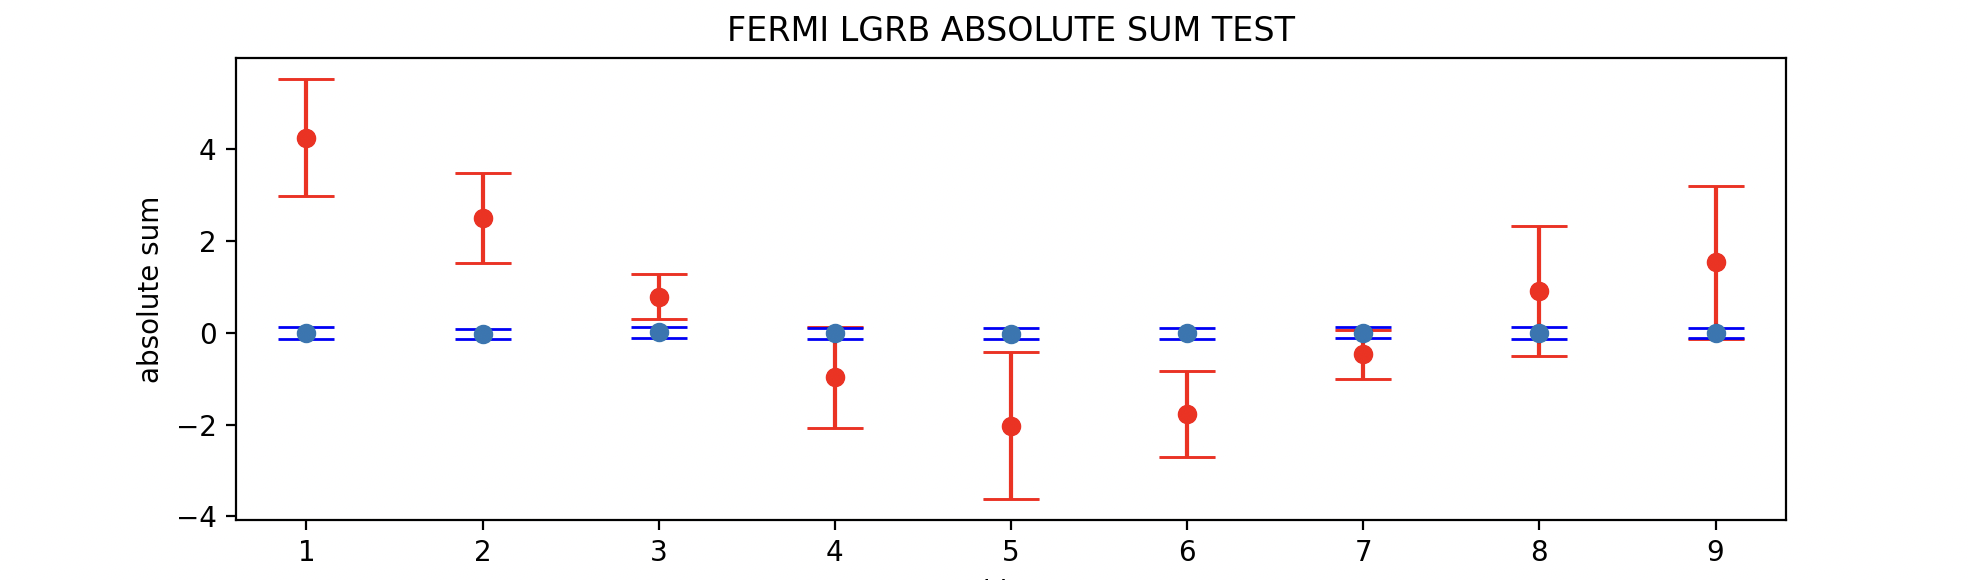
\includegraphics{FERMI LGRB sum test.png}
        \caption{The absolute sum test of the 2pACF per bin. As mentioned above, the numbers on the x axis refer to a particular bin. The red markers and bars correspond to the real data, while the blue markers and bars represent the isotropic realisations. These results are valid for the FERMI catalog LGRB sample.}
        \label{fig:enter-label}
    \end{figure}
    \begin{figure}
        \centering
        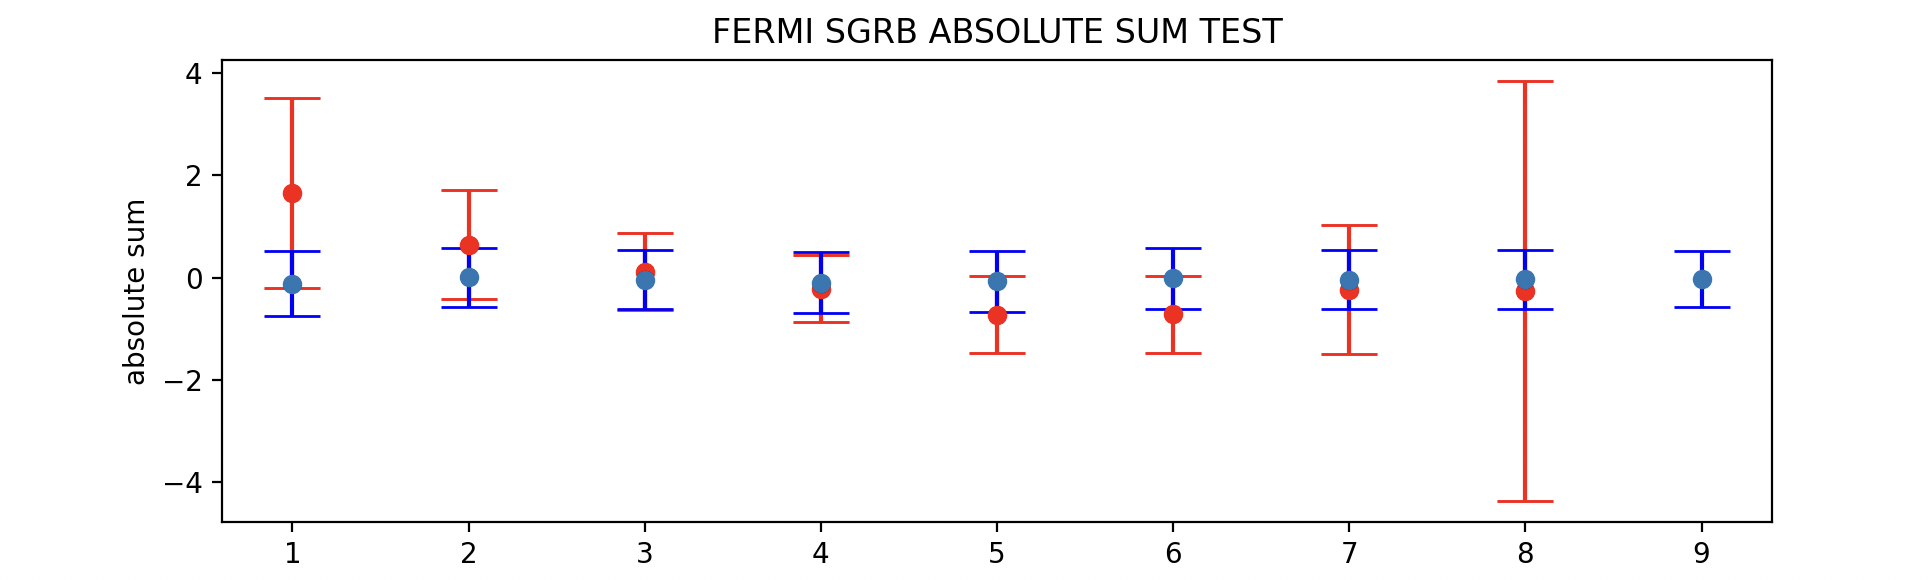
\includegraphics{FERMI SGRB sum test.png}
        \caption{Same as Figure 4, but for the FERMI SGRB sample.}
        \label{fig:enter-label}
    \end{figure}
    \end{center}
\end{quote}
\newpage
\begin{quote}
    \textbf{BATSE DATASET}\\
    \begin{center}
    \begin{figure}
        \centering
        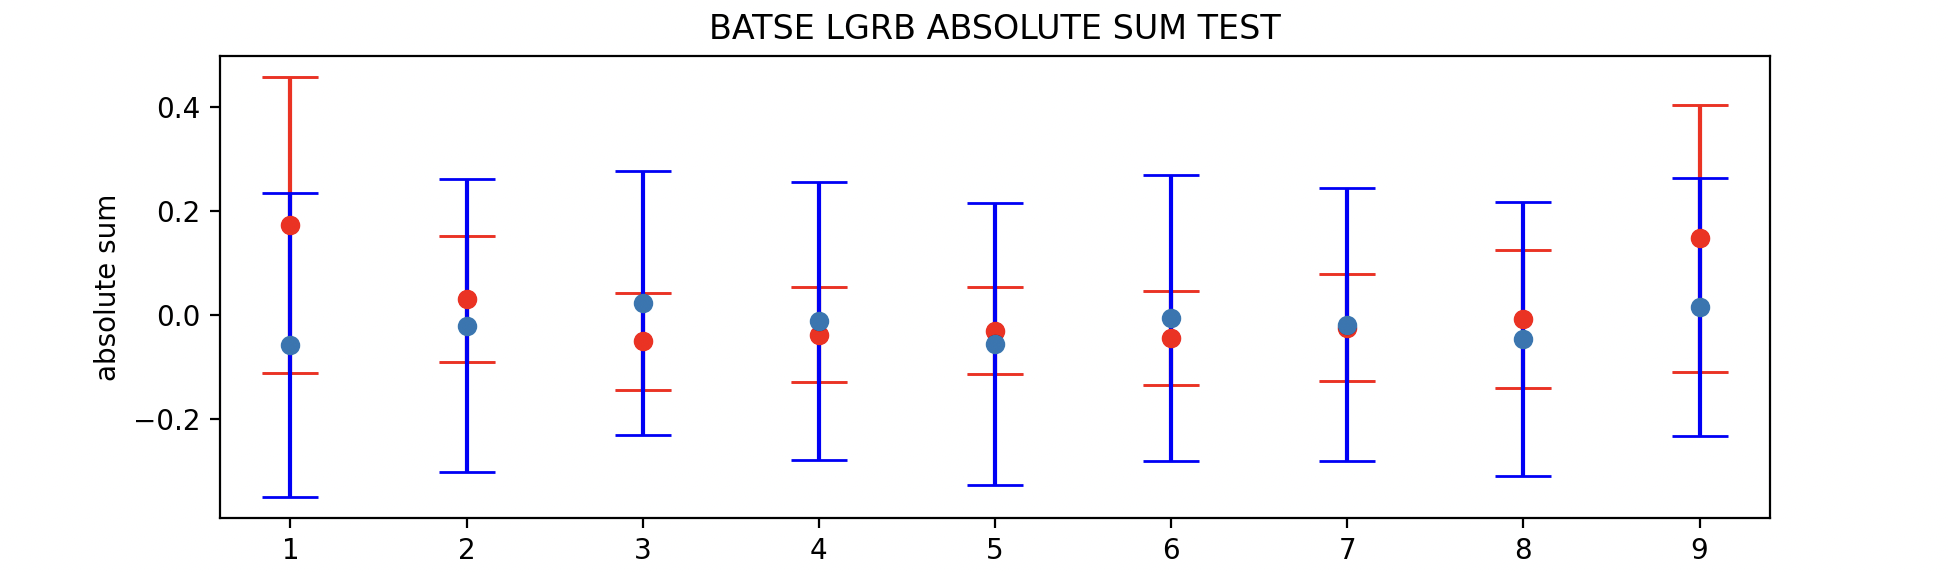
\includegraphics{BATSE LGRB sum test.png}
        \caption{Same as Figure 4, but for the BATSE LGRB sample.}
        \label{fig:enter-label}
    \end{figure}
    \begin{figure}
        \centering
        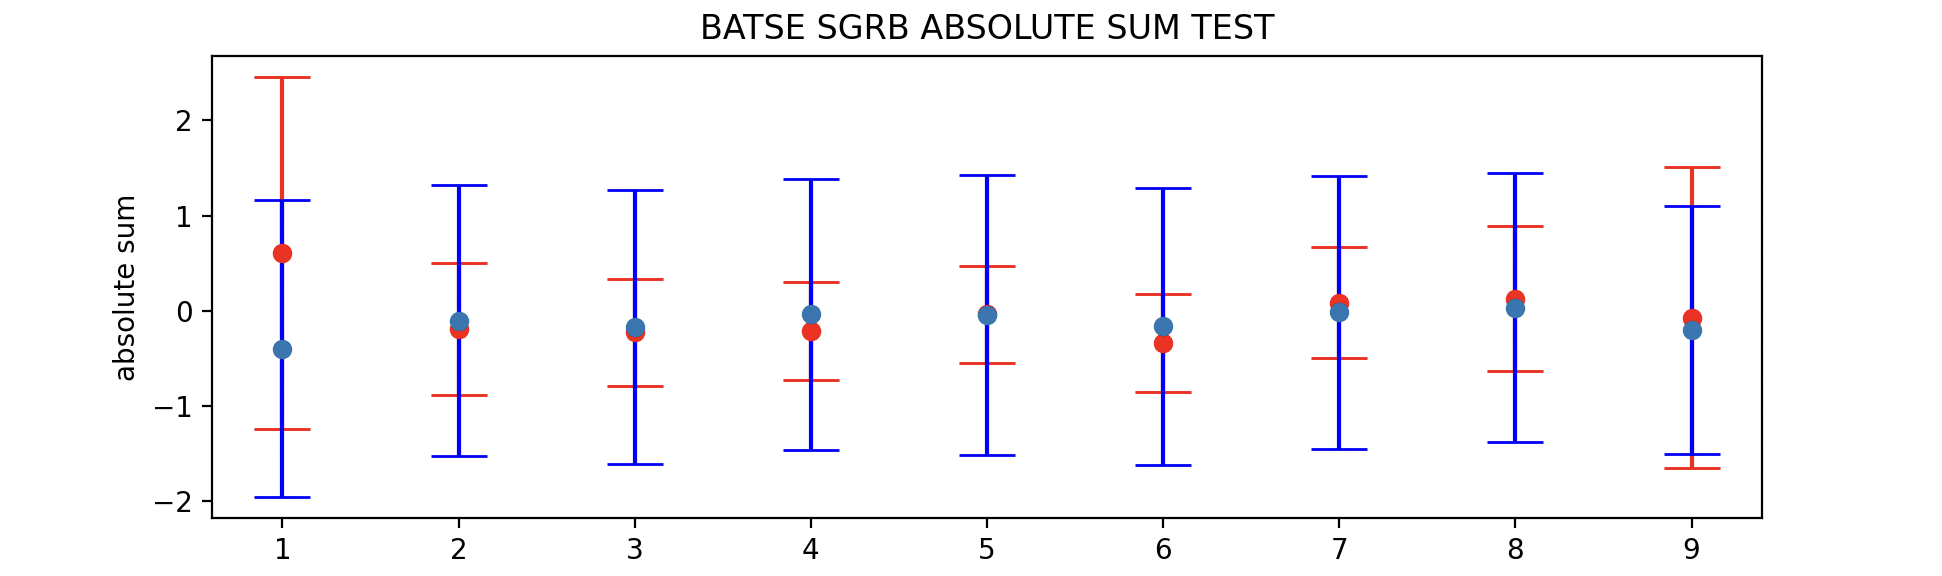
\includegraphics{BATSE SGRB sum test.png}
        \caption{Same as Figure 4, but for the BATSE SGRB sample.}
        \label{fig:enter-label}
    \end{figure}
    \end{center}
\end{quote}
\newpage
\begin{quote}
    \textbf{SWIFT DATASET}\\
    \begin{center}
    \begin{figure}
        \centering
        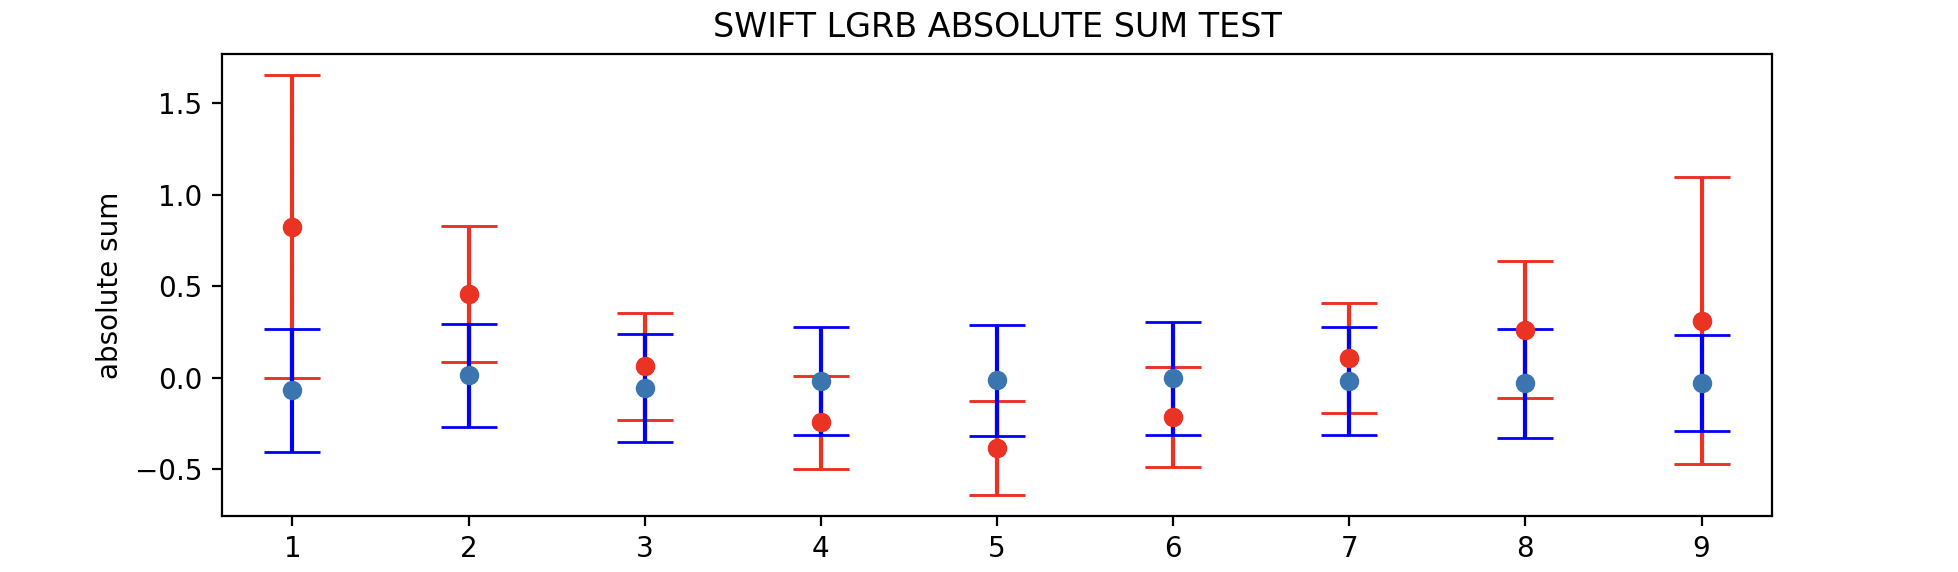
\includegraphics{SWIFT LGRB sum test.png}
        \caption{Same as Figure 4, but for the SWIFT LGRB sample.}
        \label{fig:enter-label}
    \end{figure}
    \begin{figure}
        \centering
        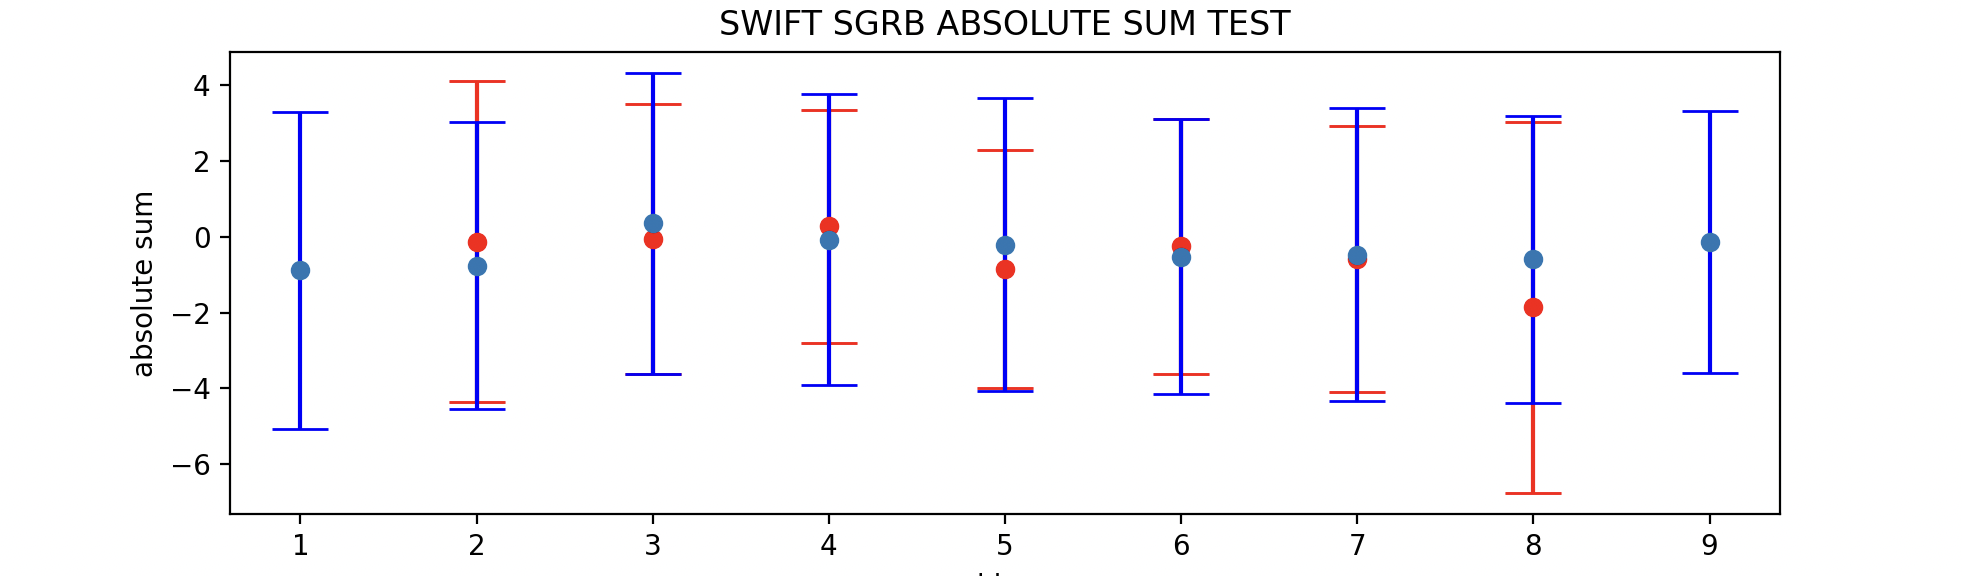
\includegraphics{SWIFT SGRB sum test.png}
        \caption{Same as Figure 4, but for the SWIFT SGRB sample.}
        \label{fig:enter-label}
    \end{figure}
    \end{center}
\end{quote}


\newpage
\textbf{\begin{enumerate}
\def\labelenumi{\arabic{enumi}.}
\setcounter{enumi}{2}
\item
  2PACF GRAPHS
\end{enumerate}
}
The following plots represent the 2pACF of the datasets. The black markers represent the value of the 2pACF at that value of \(\theta\). The shaded region represents the 2pACF of the homogeneous distribution (benchmark).\\
\begin{quote}
    \textbf{FERMI DATASET}\\
    \begin{center}
    \begin{figure}
        \centering
        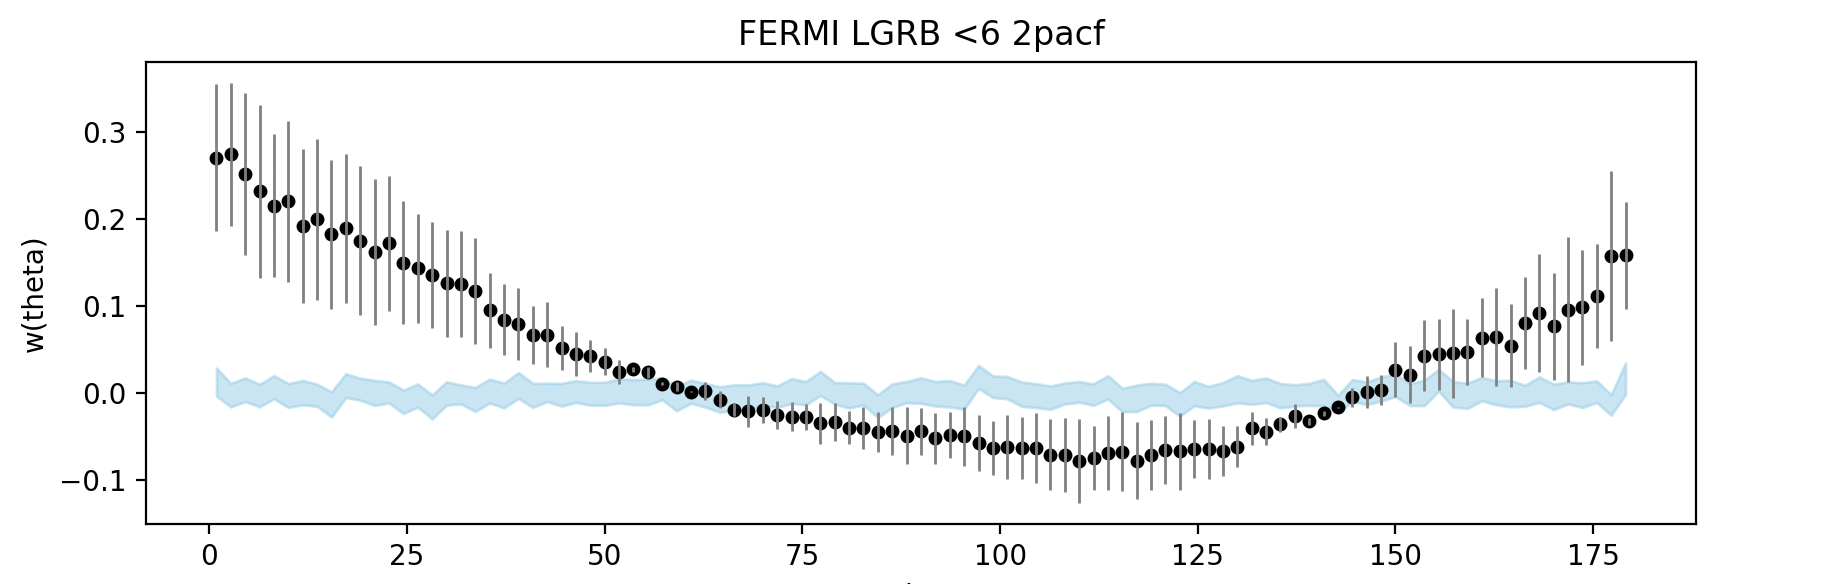
\includegraphics{FERMI LGRB 2PACFFF.png}
        \caption{The 2pACF obtained from the synthetic isotropic sample (benchmark; shaded regions), and from the LGRBs (\(T_{90} \geq 2s\)) of the Fermi catalog with \(\sigma_r \leq 6\)° (black dots).}
        \label{fig:enter-label}
    \end{figure}
    \begin{figure}
        \centering
        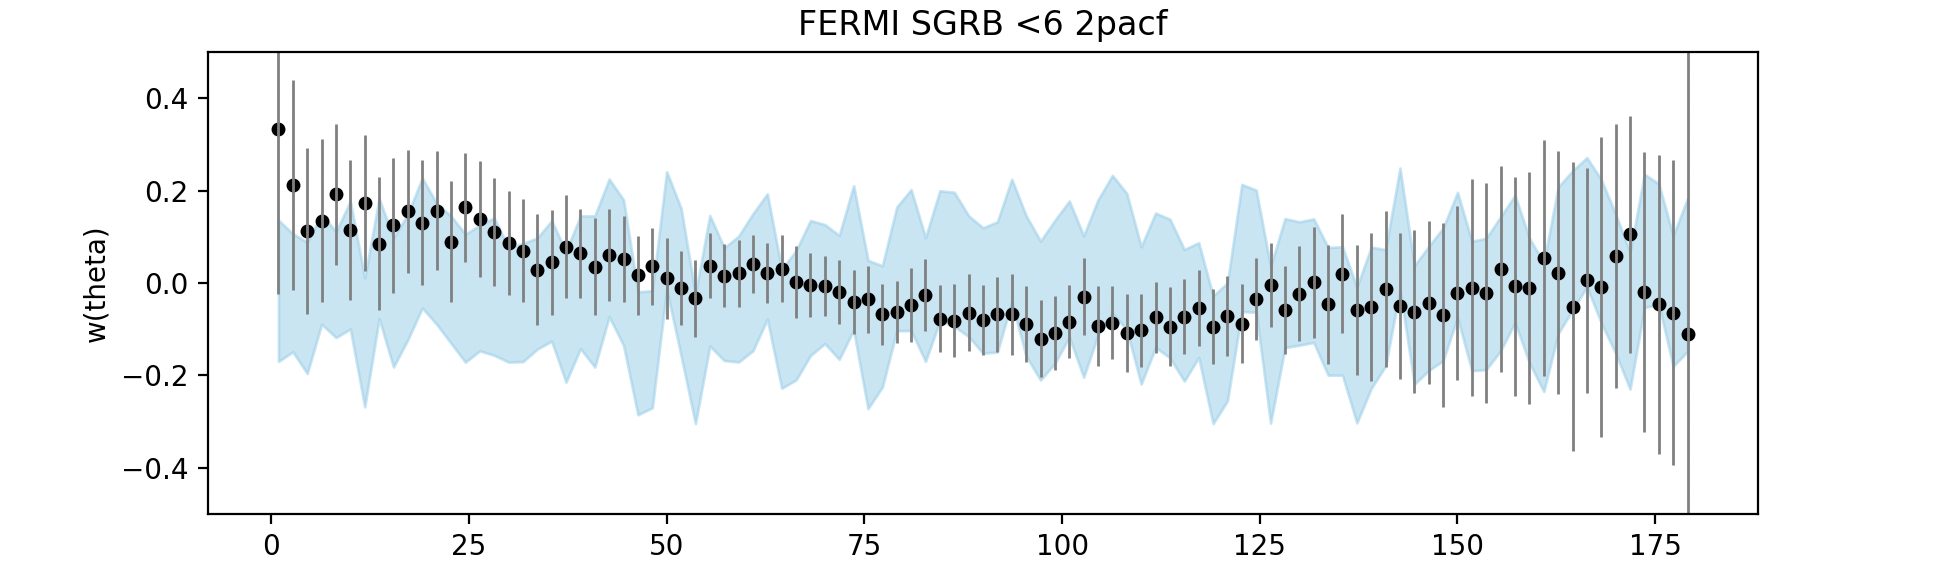
\includegraphics{FERMI SGRB 2pACF.png}
        \caption{Same as Figure 10, but for the SGRBs (\(T_{90} \leq 2s\)) of the FERMI catalog.}
        \label{fig:enter-label}
    \end{figure}
    \end{center}
\end{quote}
\newpage
\begin{quote}
    \textbf{BATSE DATASET}\\
    \begin{center}
    \begin{figure}
        \centering
        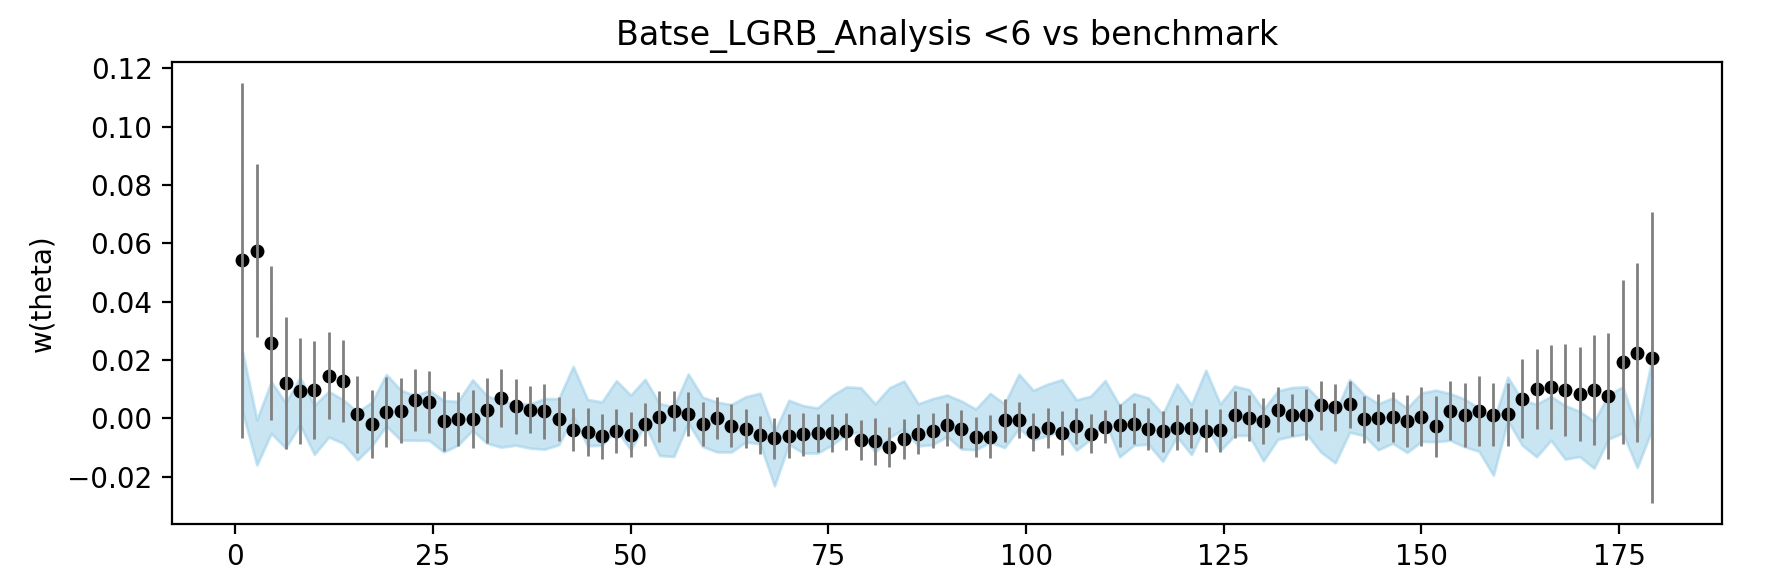
\includegraphics{BATSE LGRB 2pACF.png}
        \caption{Same as Figure 10, but for the BATSE LGRB sample.}
        \label{fig:enter-label}
    \end{figure}
    \begin{figure}
        \centering
        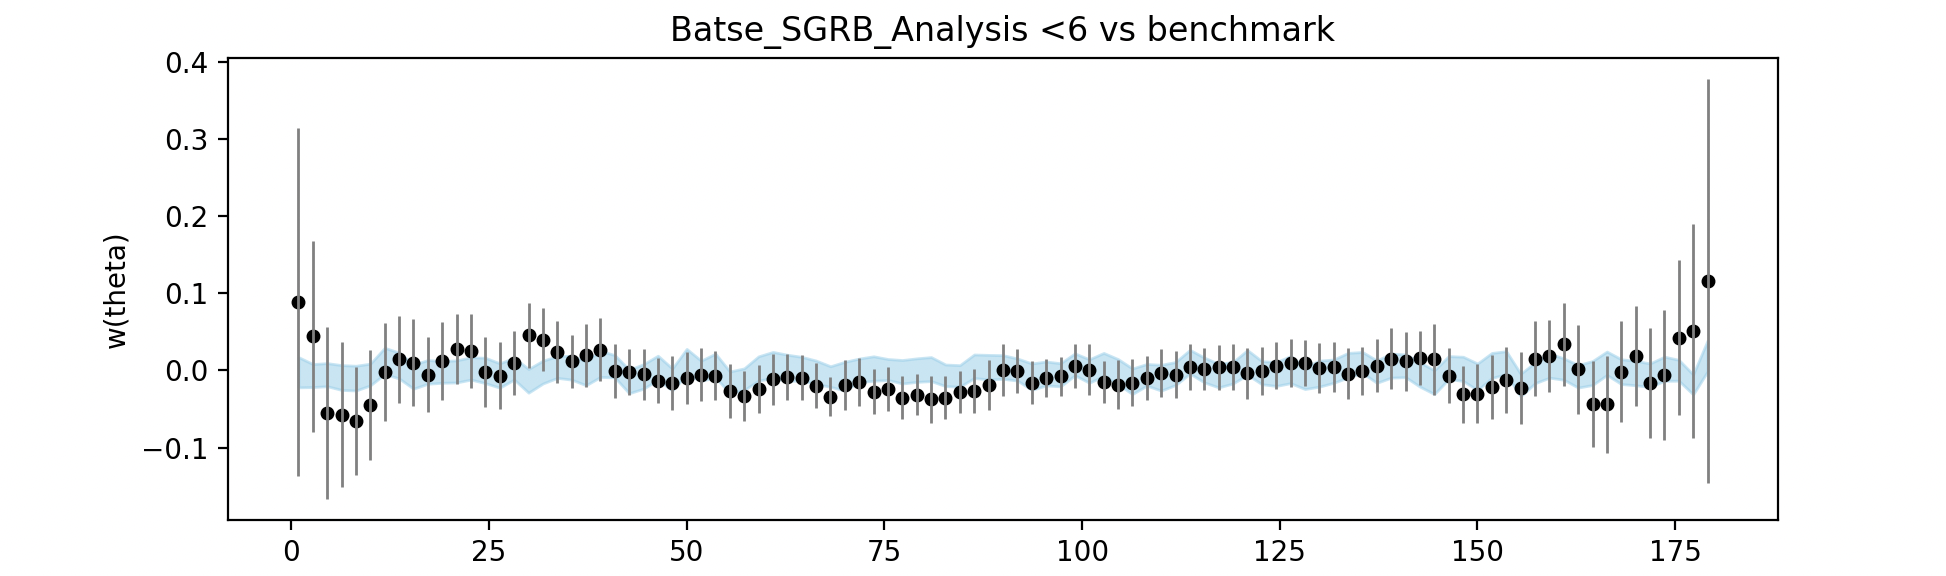
\includegraphics{BATSE SGRB 2pACF.png}
        \caption{Same as Figure 10, but for the BATSE SGRB sample.}
        \label{fig:enter-label}
    \end{figure}
    \end{center}
\end{quote}
\newpage
\begin{quote}
    \textbf{SWIFT DATASET}\\
    \begin{center}
    \begin{figure}
        \centering
        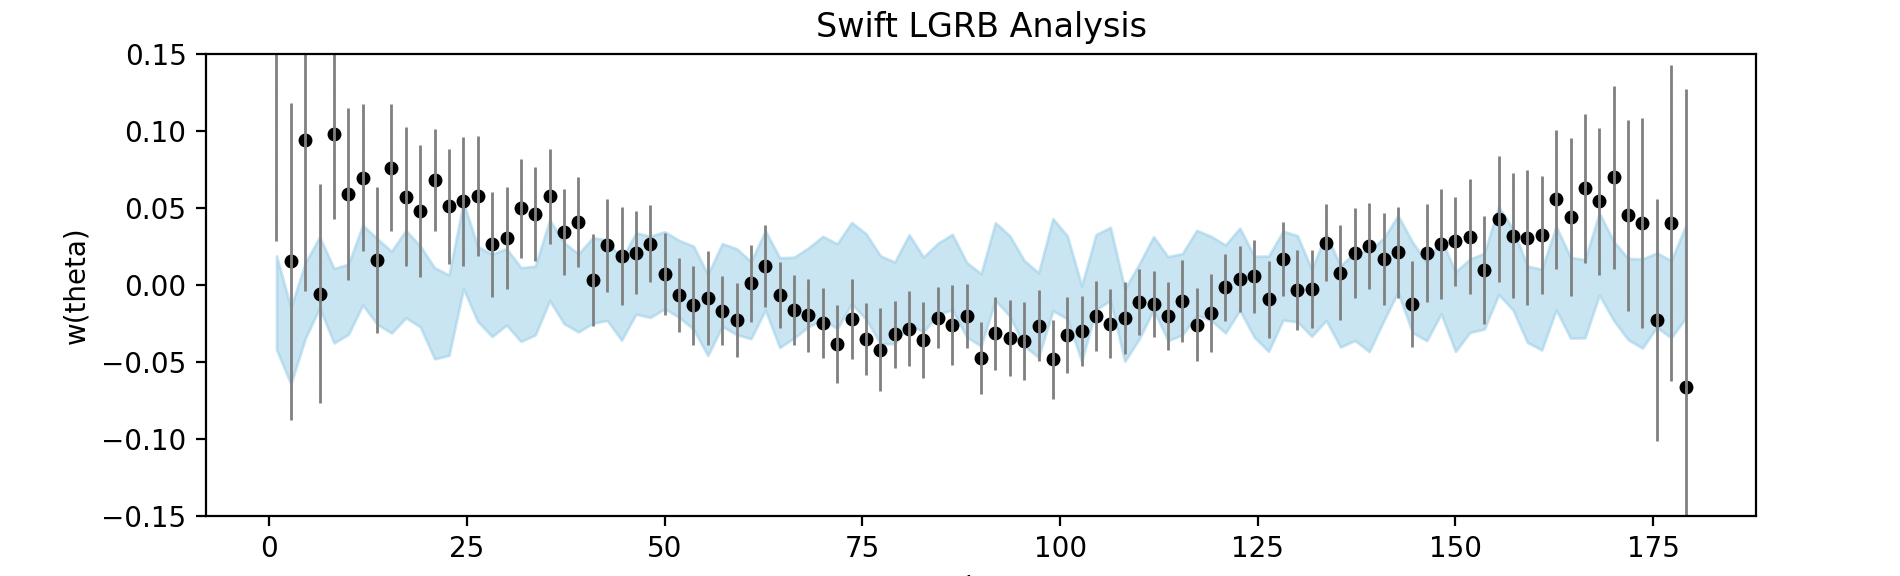
\includegraphics{Swift LGRB 2pACF1.png}
        \caption{Same as Figure 10, but for the SWIFT LGRB sample.}
        \label{fig:enter-label}
    \end{figure}
    \begin{figure}
        \centering
        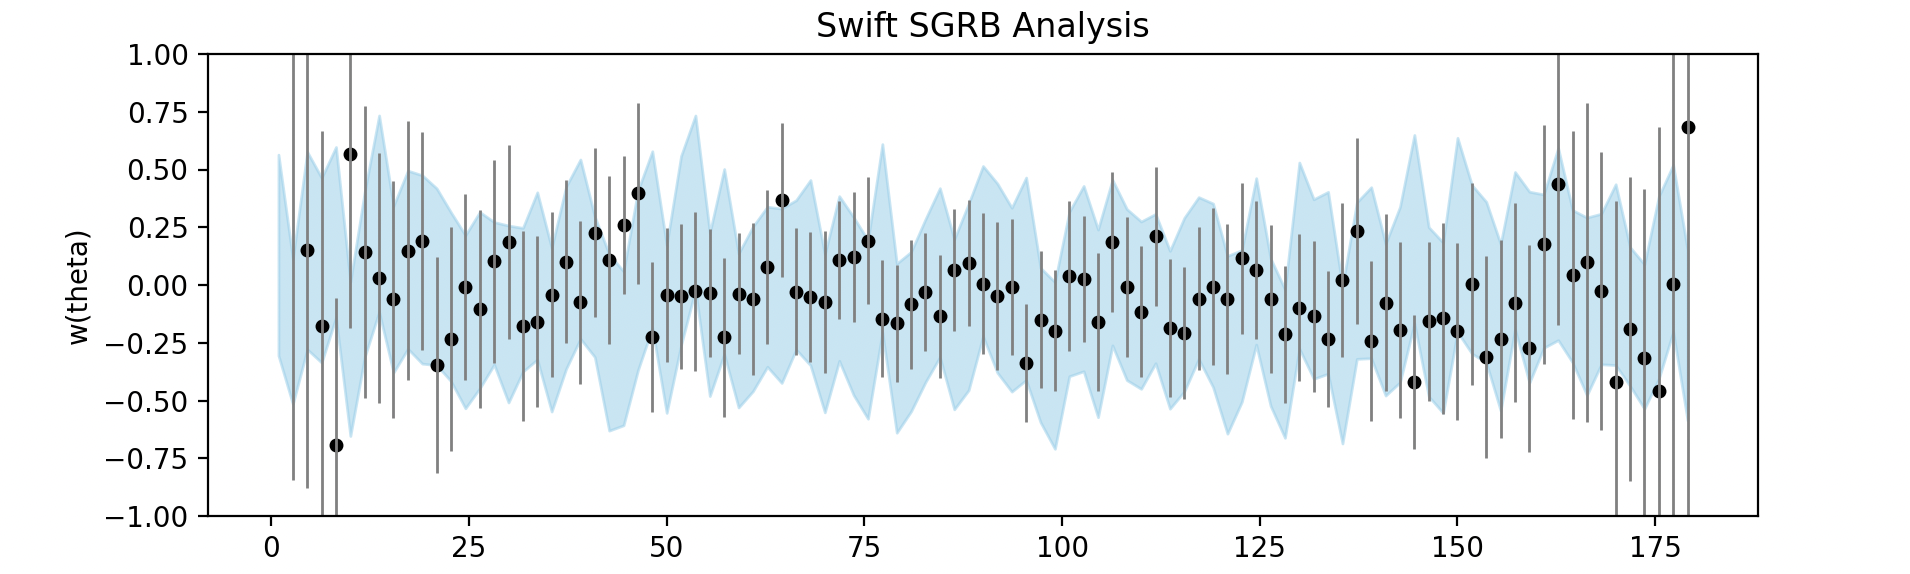
\includegraphics{Swift SGRB 2pacf1.png}
        \caption{Same as Figure 10, but for the SWIFT SGRB sample.}
        \label{fig:enter-label}
    \end{figure}
    \end{center}
\end{quote}
\newpage
\textbf{\begin{enumerate}
\def\labelenumi{\arabic{enumi}.}
\setcounter{enumi}{3}
\item
  KS and AD TEST RESULTS
\end{enumerate}
}

\textbf{Table 1 :- FERMI GRB}
Results using both the Kolmogorov-Smirnov statistic D and the Anderson-Darling statistic AD for the FERMI catalogue.

\begin{longtable}[]{@{}
  >{\raggedright\arraybackslash}p{(\columnwidth - 4\tabcolsep) * \real{0.3333}}
  >{\raggedright\arraybackslash}p{(\columnwidth - 4\tabcolsep) * \real{0.3333}}
  >{\raggedright\arraybackslash}p{(\columnwidth - 4\tabcolsep) * \real{0.3334}}@{}}
\toprule()
\begin{minipage}[b]{\linewidth}\raggedright
\end{minipage} & \begin{minipage}[b]{\linewidth}\raggedright
LGRB
\end{minipage} & \begin{minipage}[b]{\linewidth}\raggedright
SGRB
\end{minipage} \\
\midrule()
\endhead
KS statistic & 0.303030 & 0.262626 \\
KS p value & 0.000204 & 0.002069 \\
AD statistic & 13.75780 & 6.72741\\
AD p value & <0.001 & <0.001\\
\bottomrule()
\end{longtable}

\textbf{Table 2 :- BATSE GRB}
Same as Table 1, but for the BATSE GRB database

\begin{longtable}[]{@{}
  >{\raggedright\arraybackslash}p{(\columnwidth - 4\tabcolsep) * \real{0.3333}}
  >{\raggedright\arraybackslash}p{(\columnwidth - 4\tabcolsep) * \real{0.3333}}
  >{\raggedright\arraybackslash}p{(\columnwidth - 4\tabcolsep) * \real{0.3334}}@{}}
\toprule()
\begin{minipage}[b]{\linewidth}\raggedright
\end{minipage} & \begin{minipage}[b]{\linewidth}\raggedright
LGRB
\end{minipage} & \begin{minipage}[b]{\linewidth}\raggedright
SGRB
\end{minipage} \\
\midrule()
\endhead
KS statistic & 0.141414 & 0.222222 \\
KS p value & 0.276459 & 0.01482 \\
AD statistic & 1.209753 & 6.70679 \\
AD p value & 0.103225 & <0.001 \\
\bottomrule()
\end{longtable}

\textbf{Table 3 :- SWIFT GRB}
Same as Table 1, but for the SWIFT GRB database.

\begin{longtable}[]{@{}
  >{\raggedright\arraybackslash}p{(\columnwidth - 4\tabcolsep) * \real{0.3333}}
  >{\raggedright\arraybackslash}p{(\columnwidth - 4\tabcolsep) * \real{0.3333}}
  >{\raggedright\arraybackslash}p{(\columnwidth - 4\tabcolsep) * \real{0.3334}}@{}}
\toprule()
\begin{minipage}[b]{\linewidth}\raggedright
\end{minipage} & \begin{minipage}[b]{\linewidth}\raggedright
LGRB
\end{minipage} & \begin{minipage}[b]{\linewidth}\raggedright
SGRB
\end{minipage} \\
\midrule()
\endhead
KS statistic & 0.424242 & 0.090909 \\
KS p value & \(2.26*10^{-8}\) & 0.810627 \\
AD statistic & 18.47252 & 0.101597 \\
AD p value & <0.001 & >0.25 \\
\bottomrule()
\end{longtable}

\newpage
\textbf{\begin{enumerate}
\def\labelenumi{\arabic{enumi}.}
\setcounter{enumi}{4}
\item
  3D PLOTS OF DATASETS
\end{enumerate}
}
\begin{figure}[h]
  \begin{subfigure}{.5\textwidth}
  \centering
    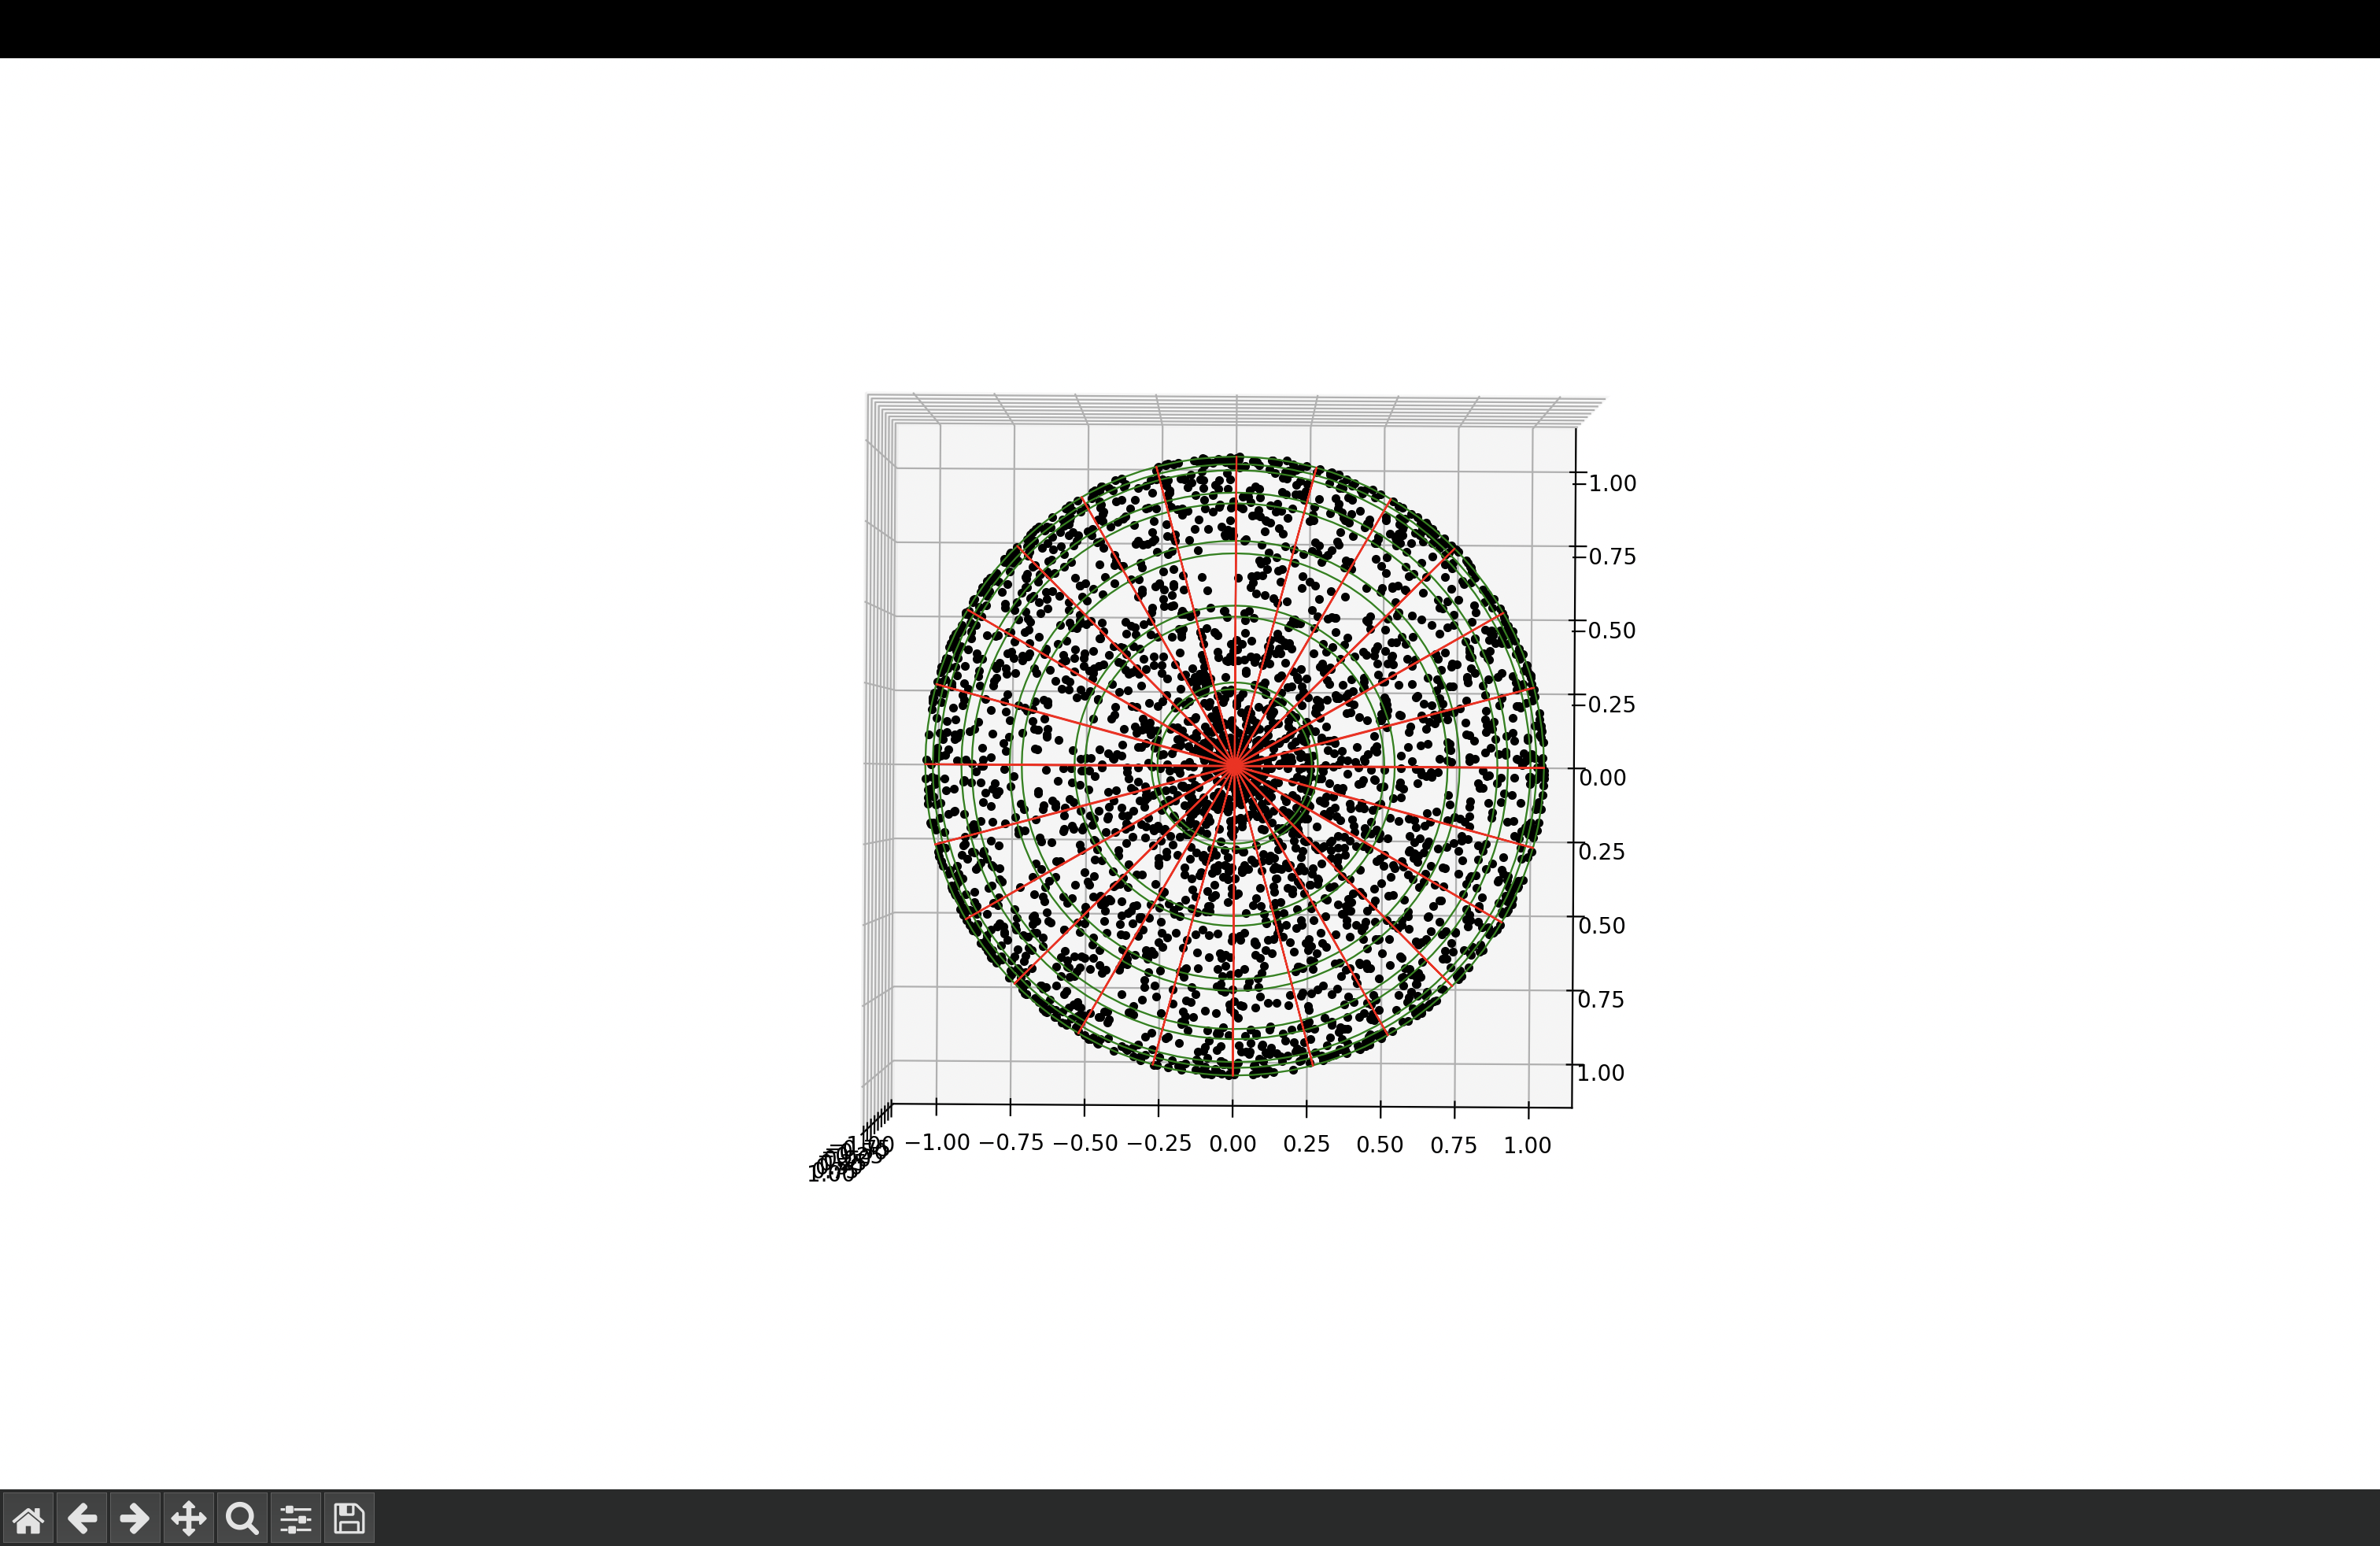
\includegraphics[width=1\linewidth]{LGRB fermi.png}
    \caption{TOP VIEW}
  \end{subfigure}%
  \begin{subfigure}{.5\textwidth}
  \centering
    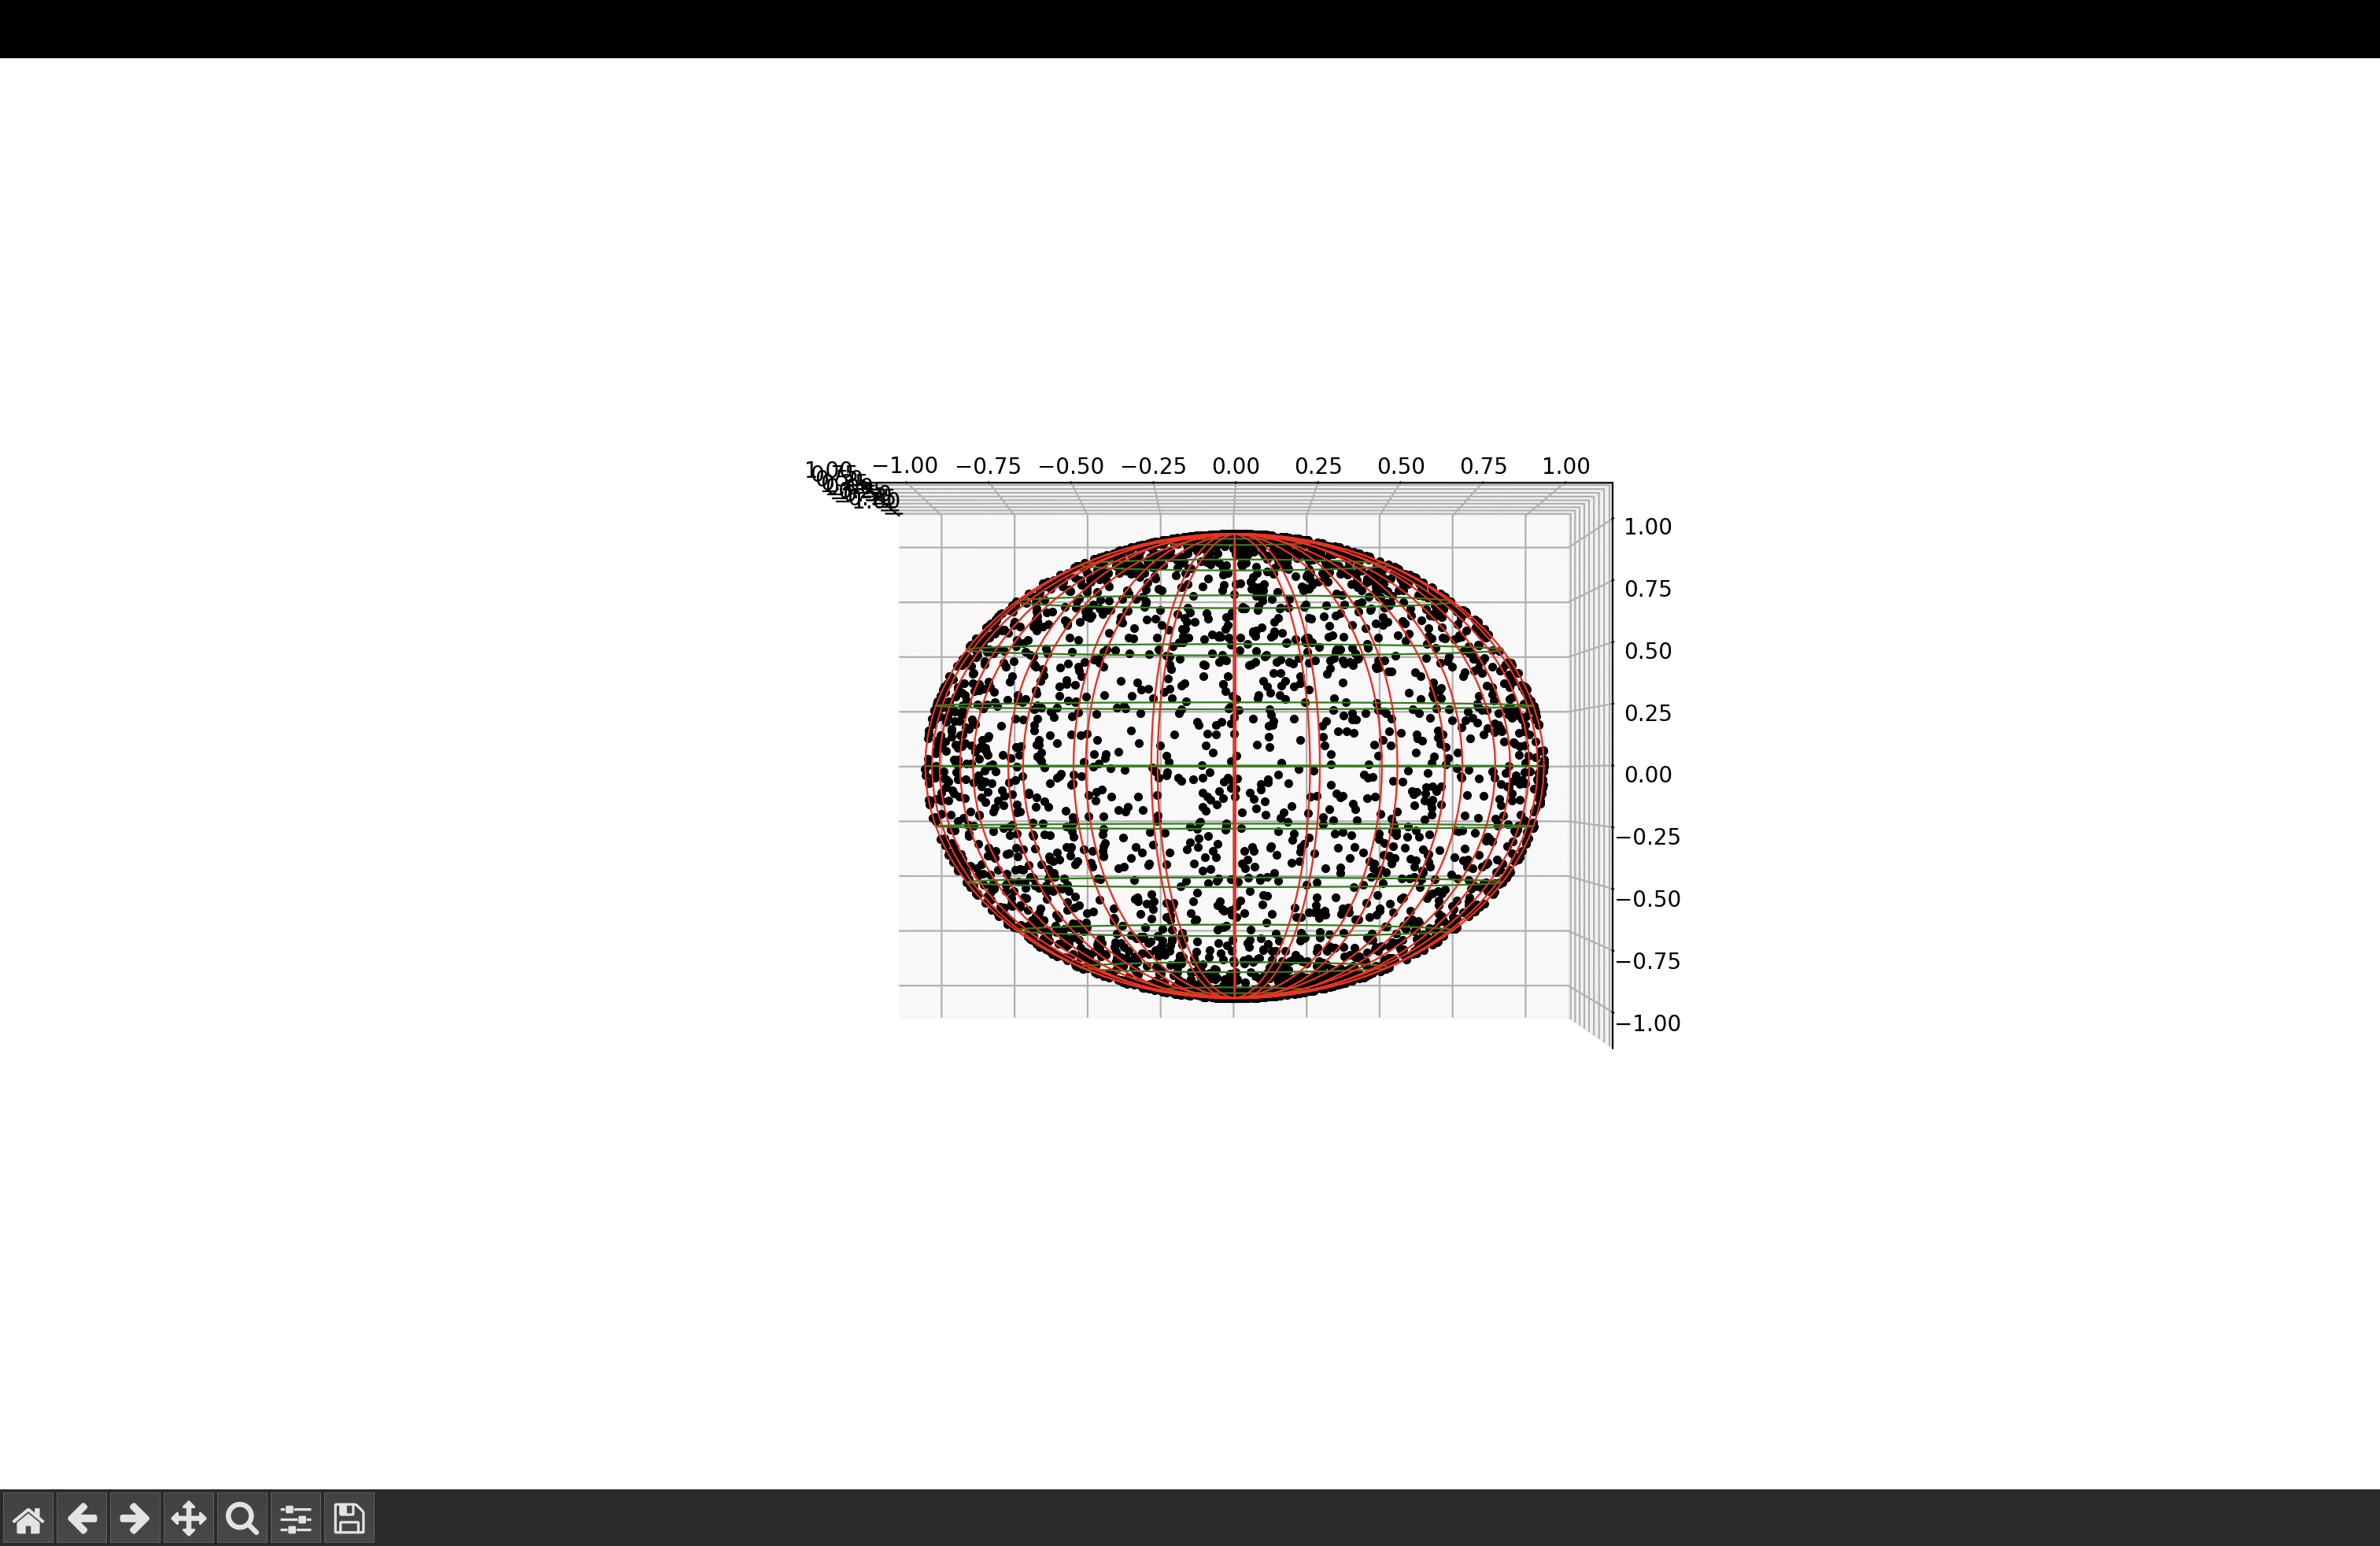
\includegraphics[width=1\linewidth]{LGRB fermii.png}
    \caption{SIDE VIEW}
  \end{subfigure}
  \caption{3D Plot of the FERMI LGRB. Clustering can be observed at the top and bottom, which confirms the results of the absolute sum test and the plot of the 2pACF function.}
\end{figure}
\begin{figure}[h]
  \begin{subfigure}{.5\textwidth}
  \centering
    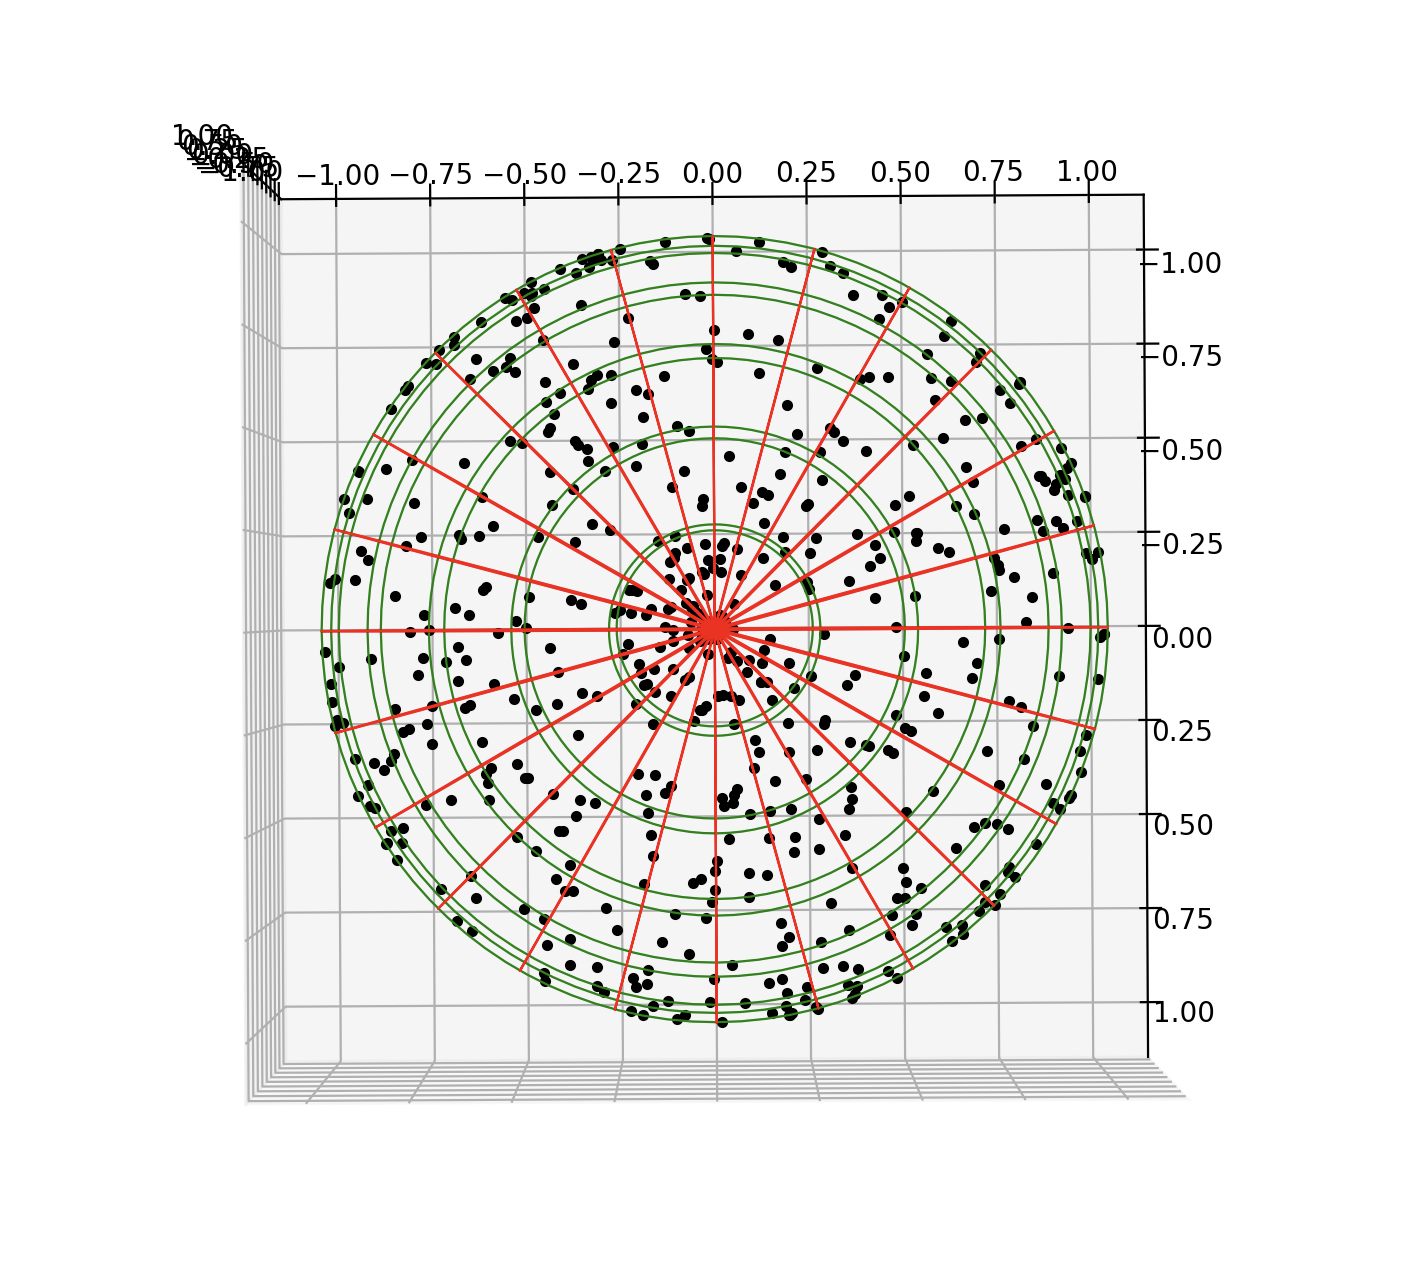
\includegraphics[width=1\linewidth]{FERMI SGRB 3D.png}
    \caption{TOP VIEW}
  \end{subfigure}%
  \begin{subfigure}{.5\textwidth}
  \centering
    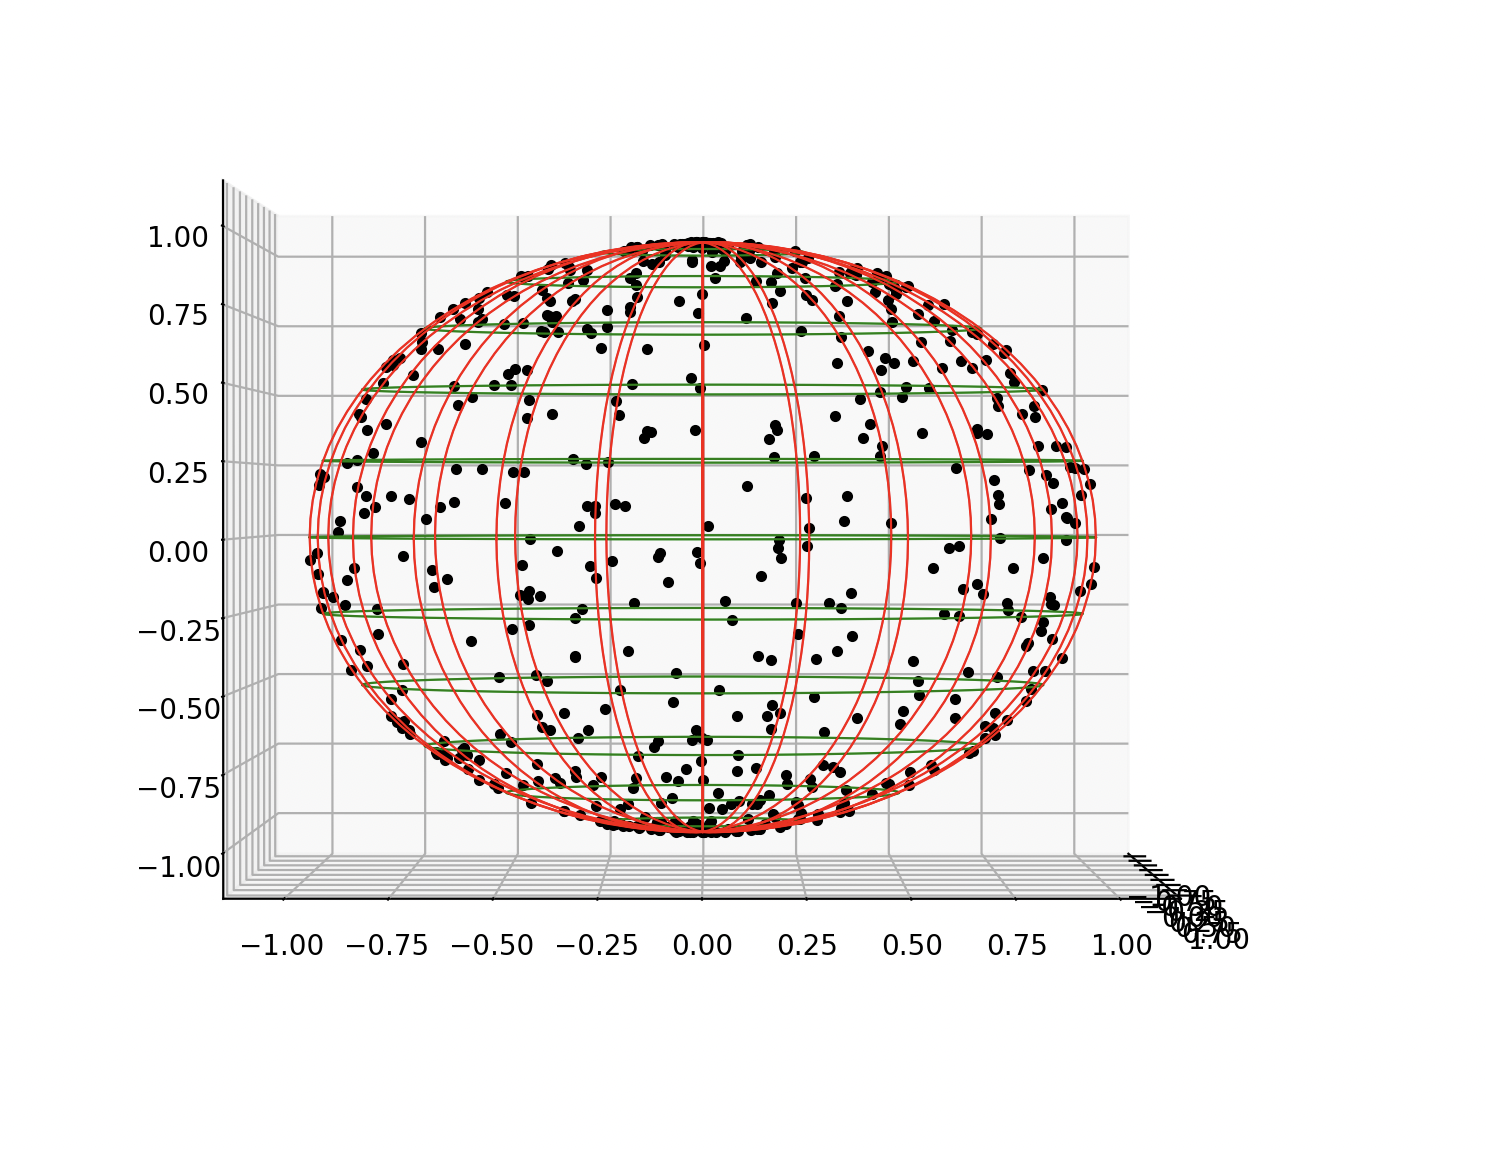
\includegraphics[width=1\linewidth]{FERMI SGRB 3DD.png}
    \caption{SIDE VIEW}
  \end{subfigure}
  \caption{3D Plot of the FERMI SGRB. Relatively not as much clustering as compared to the FERMI LGRB sample.}
\end{figure}
\begin{figure}[h]
  \begin{subfigure}{.5\textwidth}
  \centering
    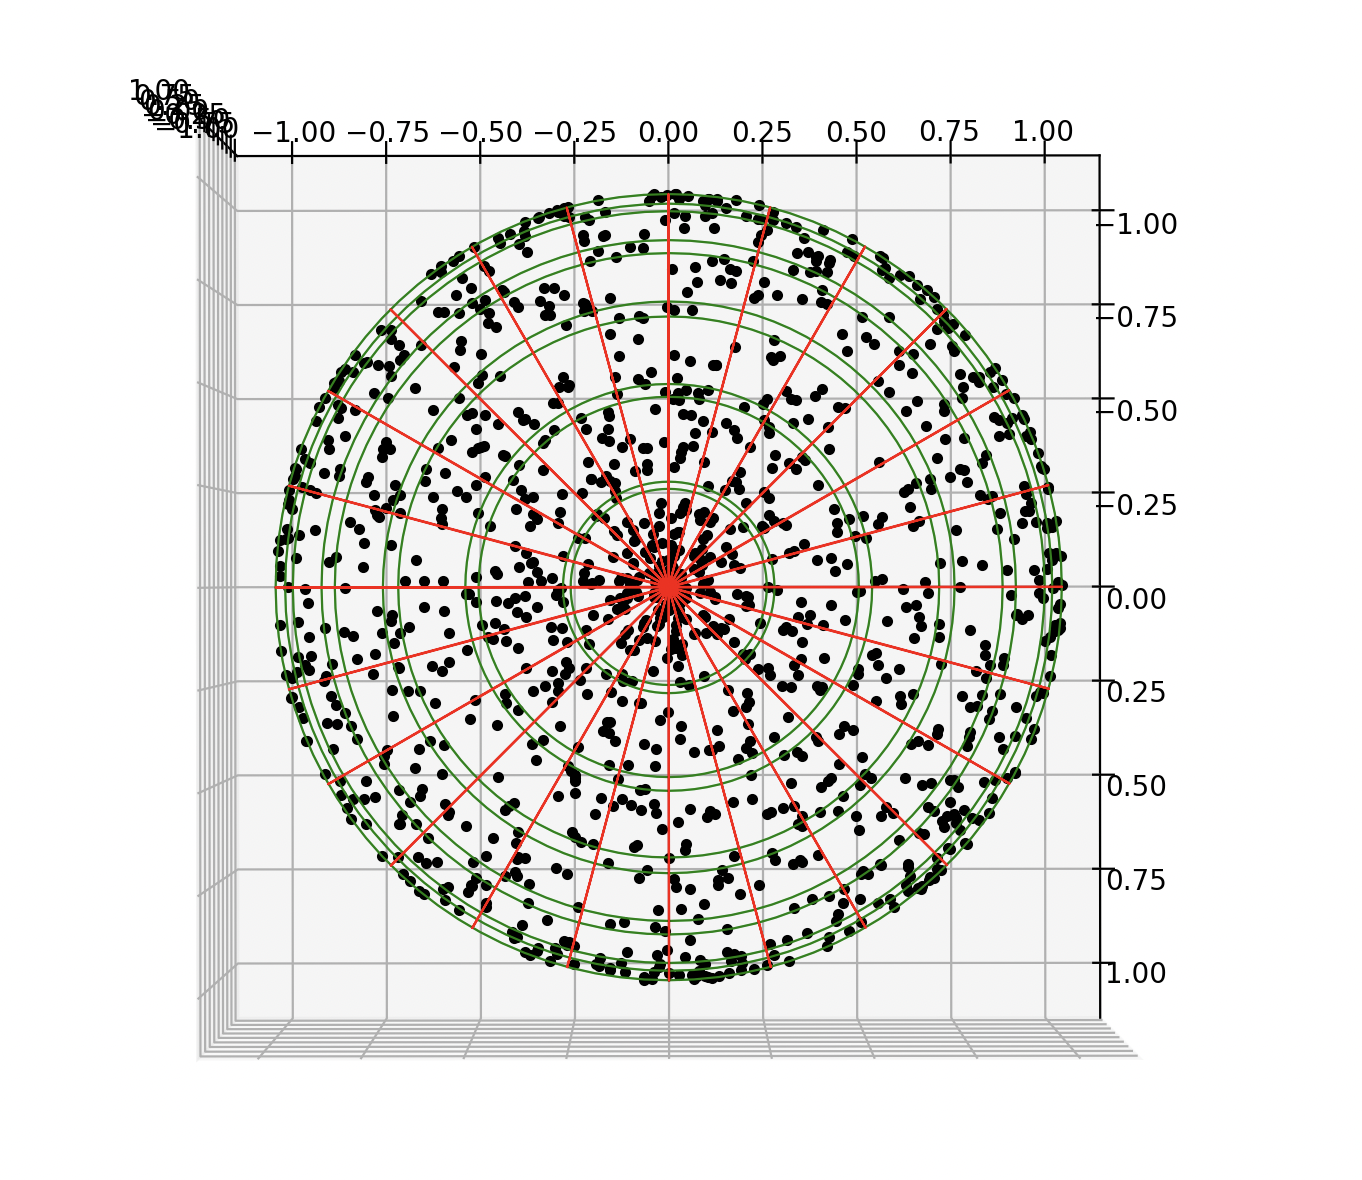
\includegraphics[width=1\linewidth]{BATSE LGRB 3D.png}
    \caption{TOP VIEW}
  \end{subfigure}%
  \begin{subfigure}{.5\textwidth}
  \centering
    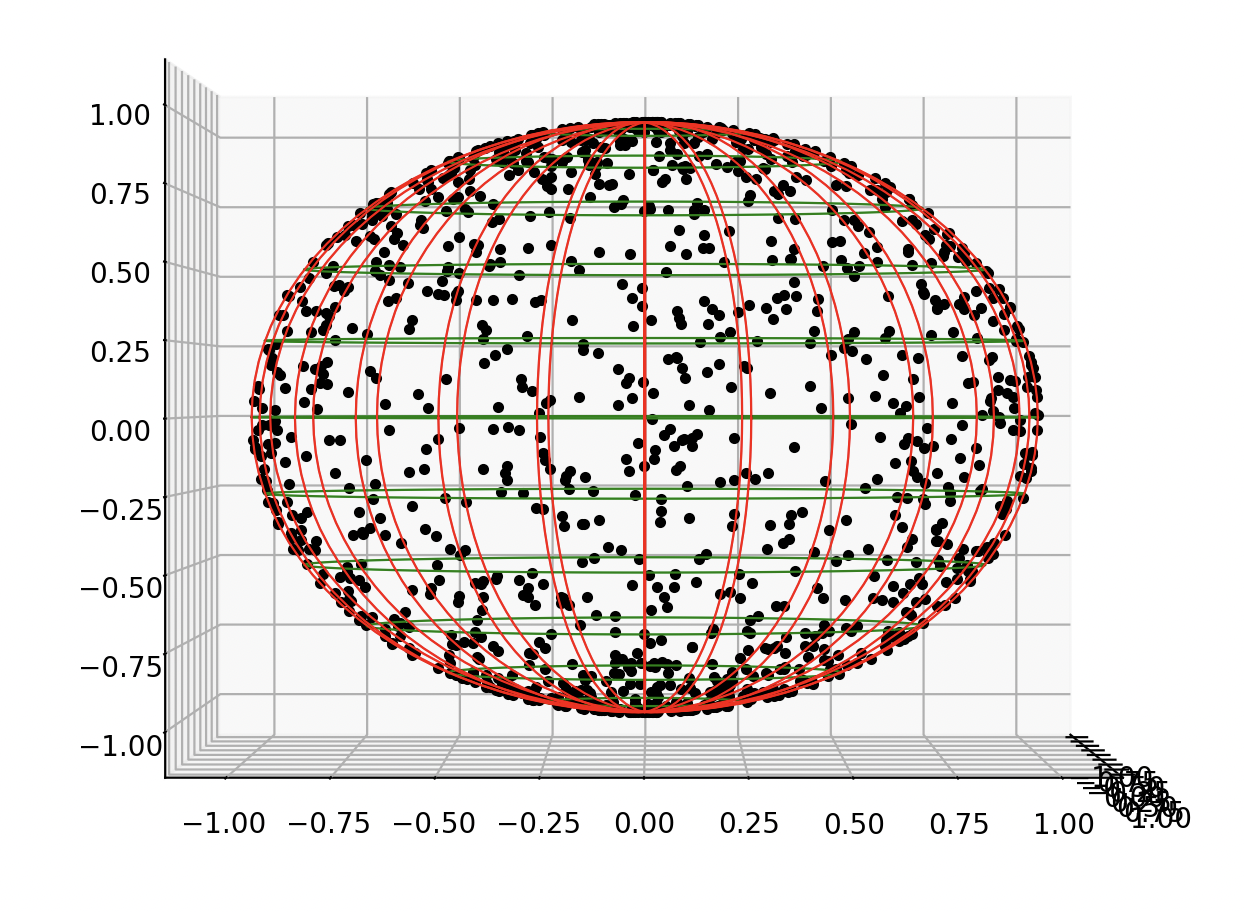
\includegraphics[width=1\linewidth]{BATSE LGRB 3DD.png}
    \caption{SIDE VIEW}
  \end{subfigure}
  \caption{3D plot of the BATSE LGRB sample. Much closer to a homogeneous distribution than the FERMI LGRB smample.}
\end{figure}
\begin{figure}[h]
  \begin{subfigure}{.5\textwidth}
  \centering
    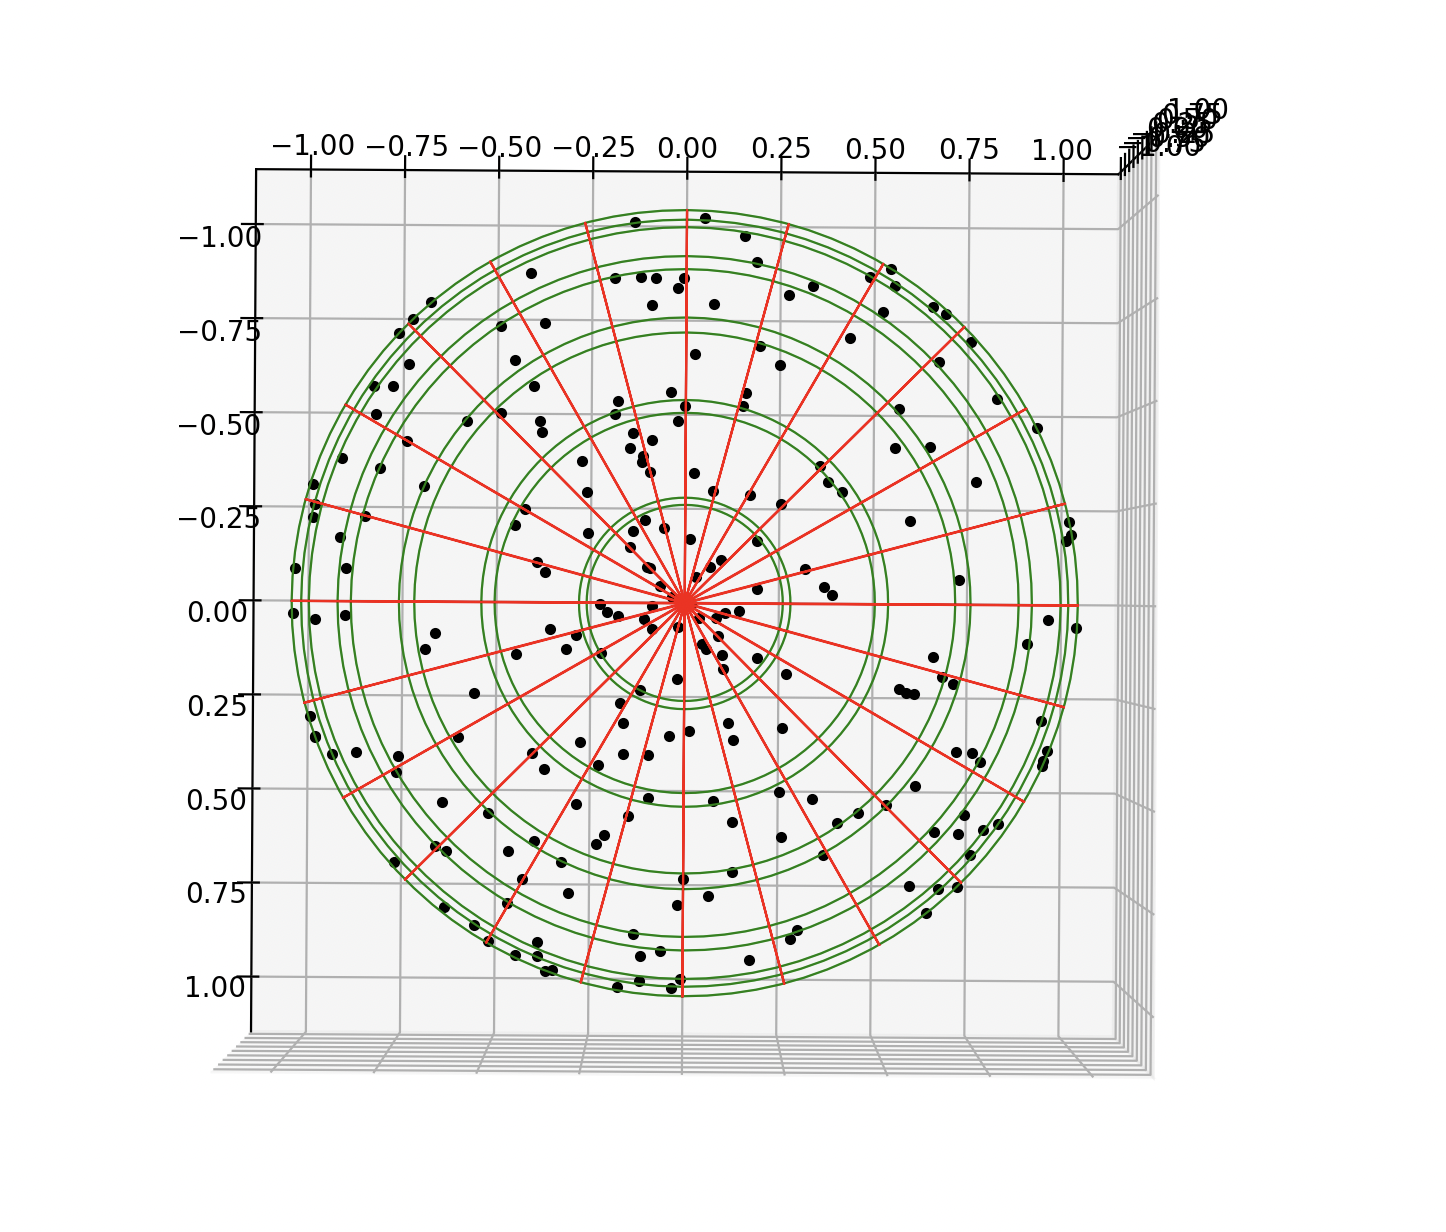
\includegraphics[width=1\linewidth]{BATSE SGRB 3D.png}
    \caption{TOP VIEW}
  \end{subfigure}%
  \begin{subfigure}{.5\textwidth}
  \centering
    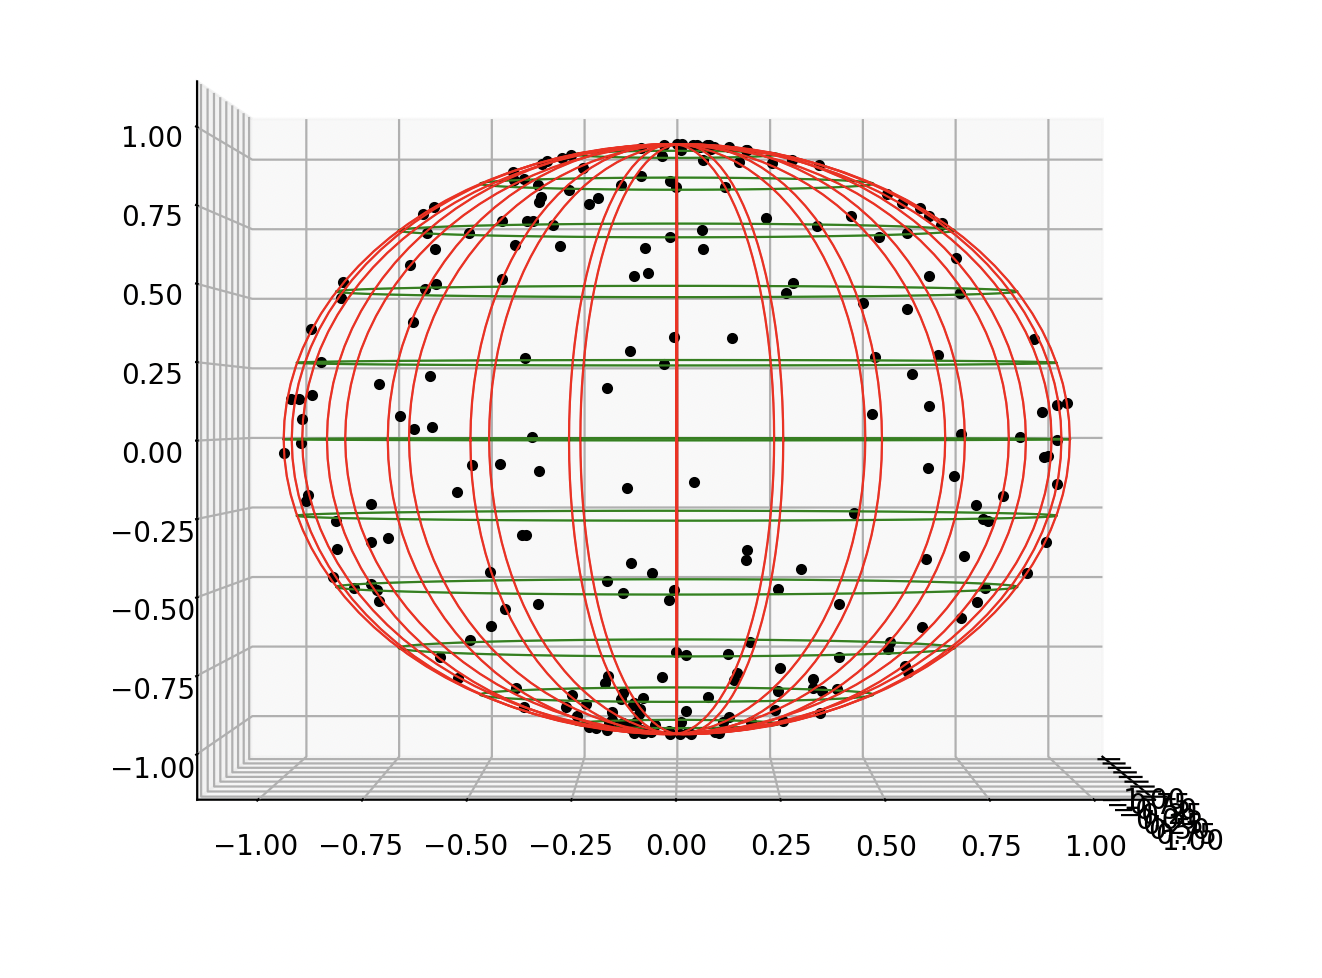
\includegraphics[width=1\linewidth]{BATSE SGRB 3DD.png}
    \caption{SIDE VIEW}
  \end{subfigure}
  \caption{3D plot of the BATSE SGRB sample. Results confirm that it is not a homogeneous distribution.}
\end{figure}
\begin{figure}[h]
  \begin{subfigure}{.5\textwidth}
  \centering
    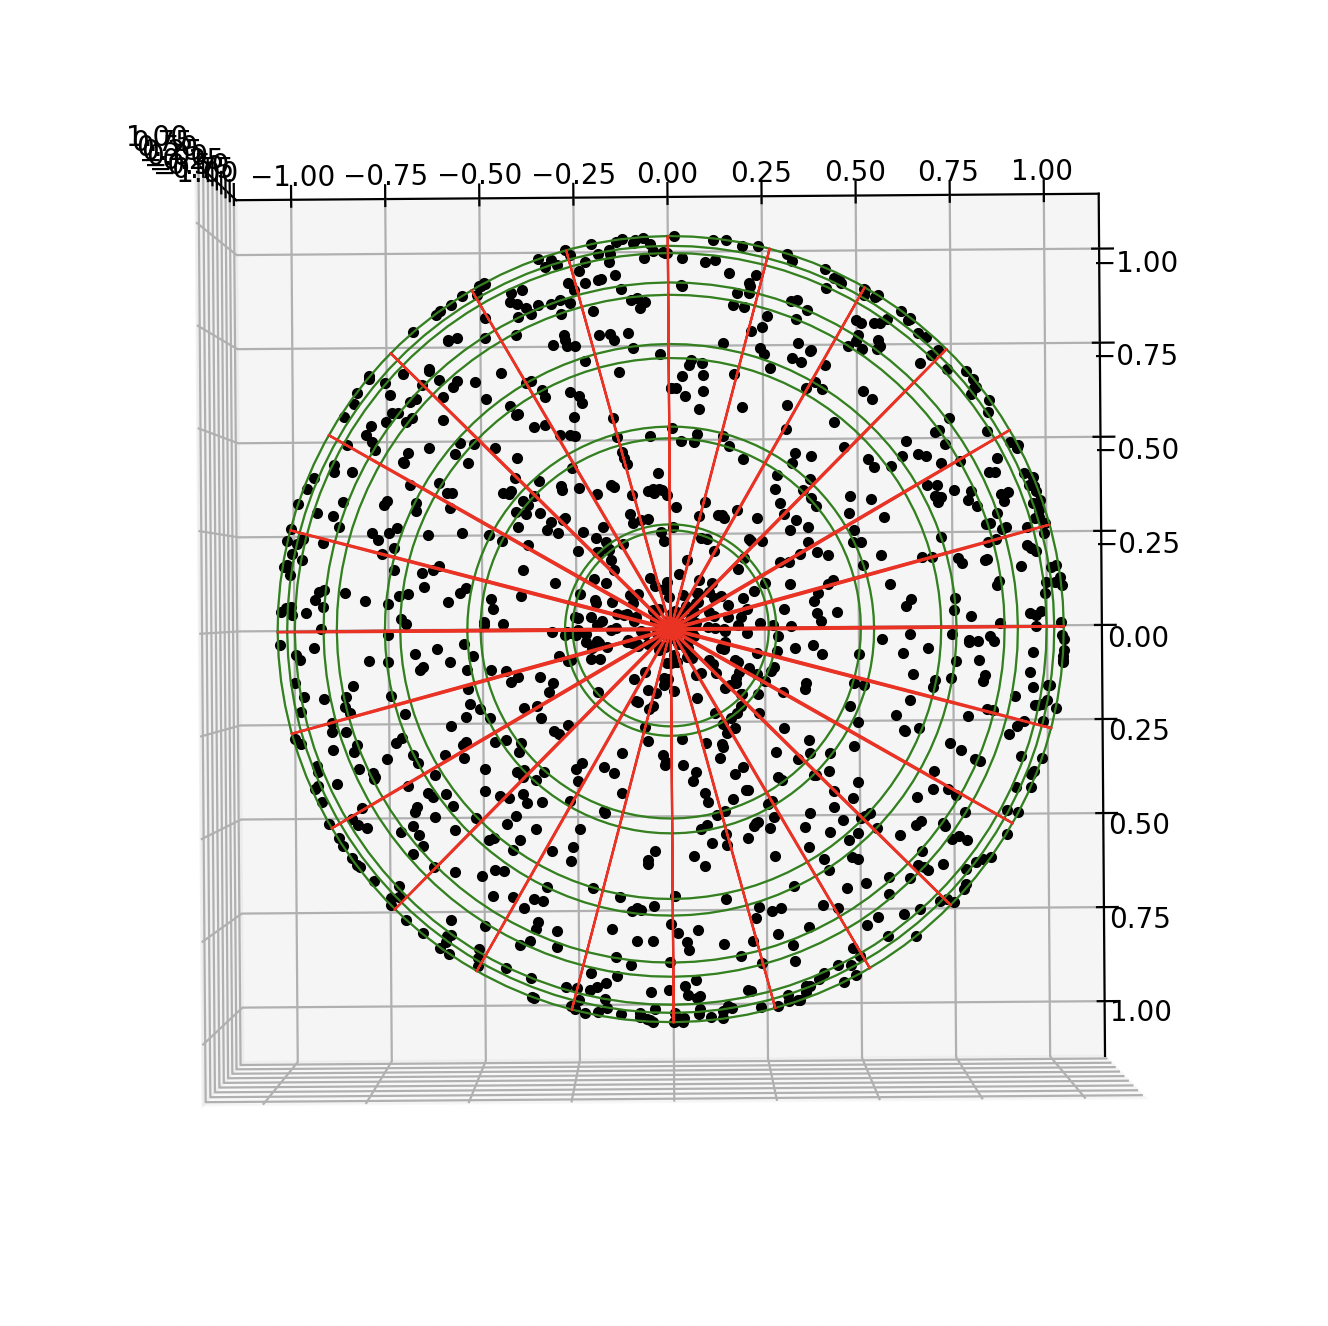
\includegraphics[width=1\linewidth]{SWIFT LGRB 3D.png}
    \caption{TOP VIEW}
  \end{subfigure}%
  \begin{subfigure}{.5\textwidth}
  \centering
    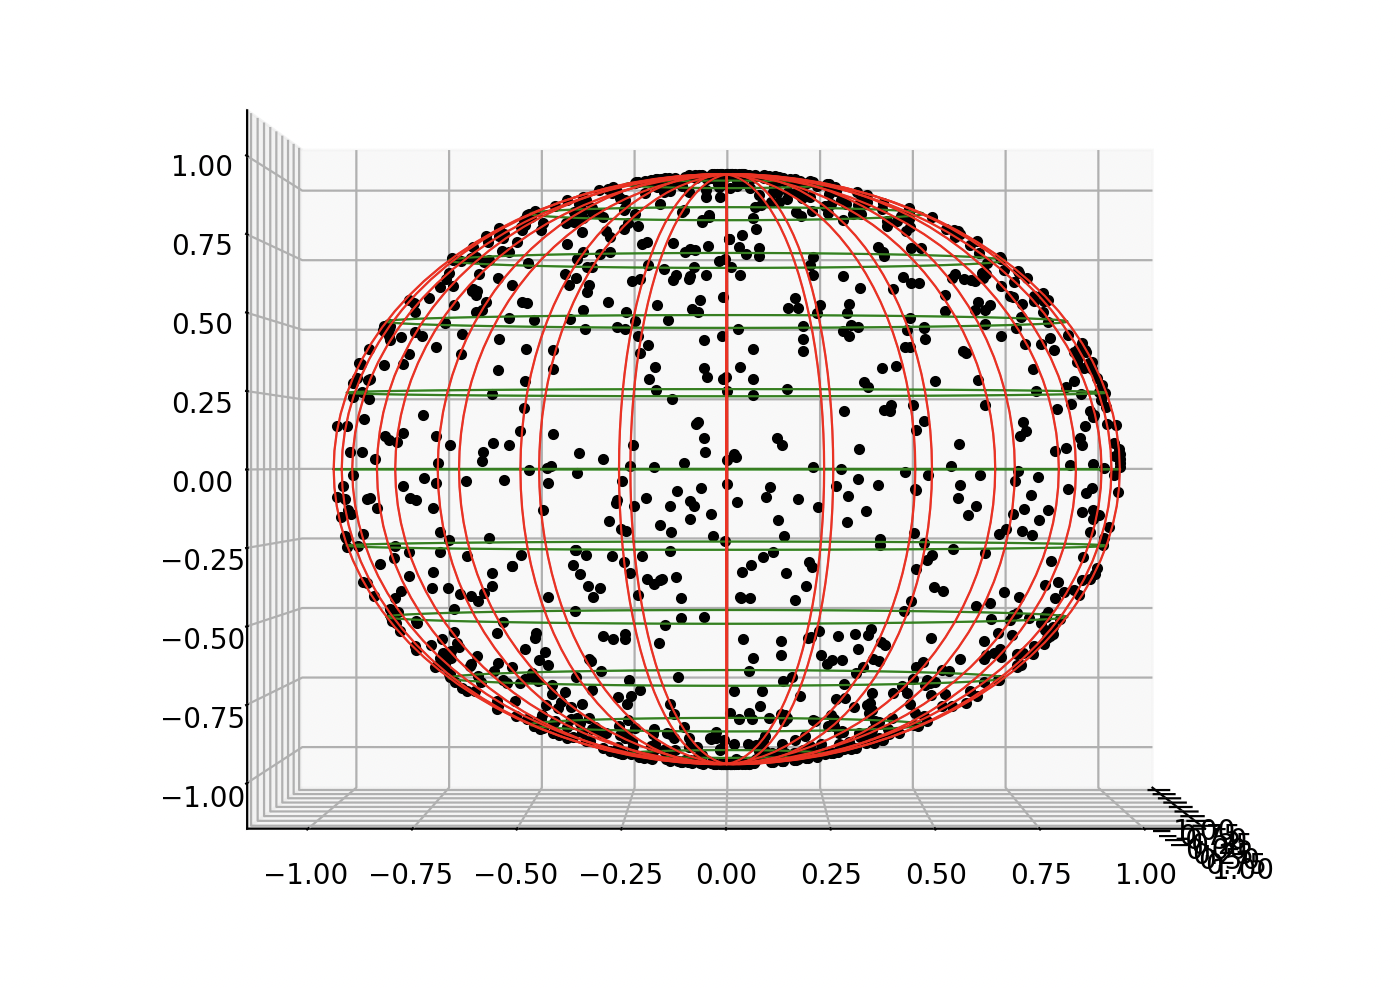
\includegraphics[width=1\linewidth]{SWIFT LGRB 3DD.png}
    \caption{SIDE VIEW}
  \end{subfigure}
  \caption{3D plot of the SWIFT LGRB sample. Deviates a bit from the isotropic homogeneous distribution but not as much as the FERMI LGRB sample}
\end{figure}
\begin{figure}[h]
  \begin{subfigure}{.5\textwidth}
  \centering
    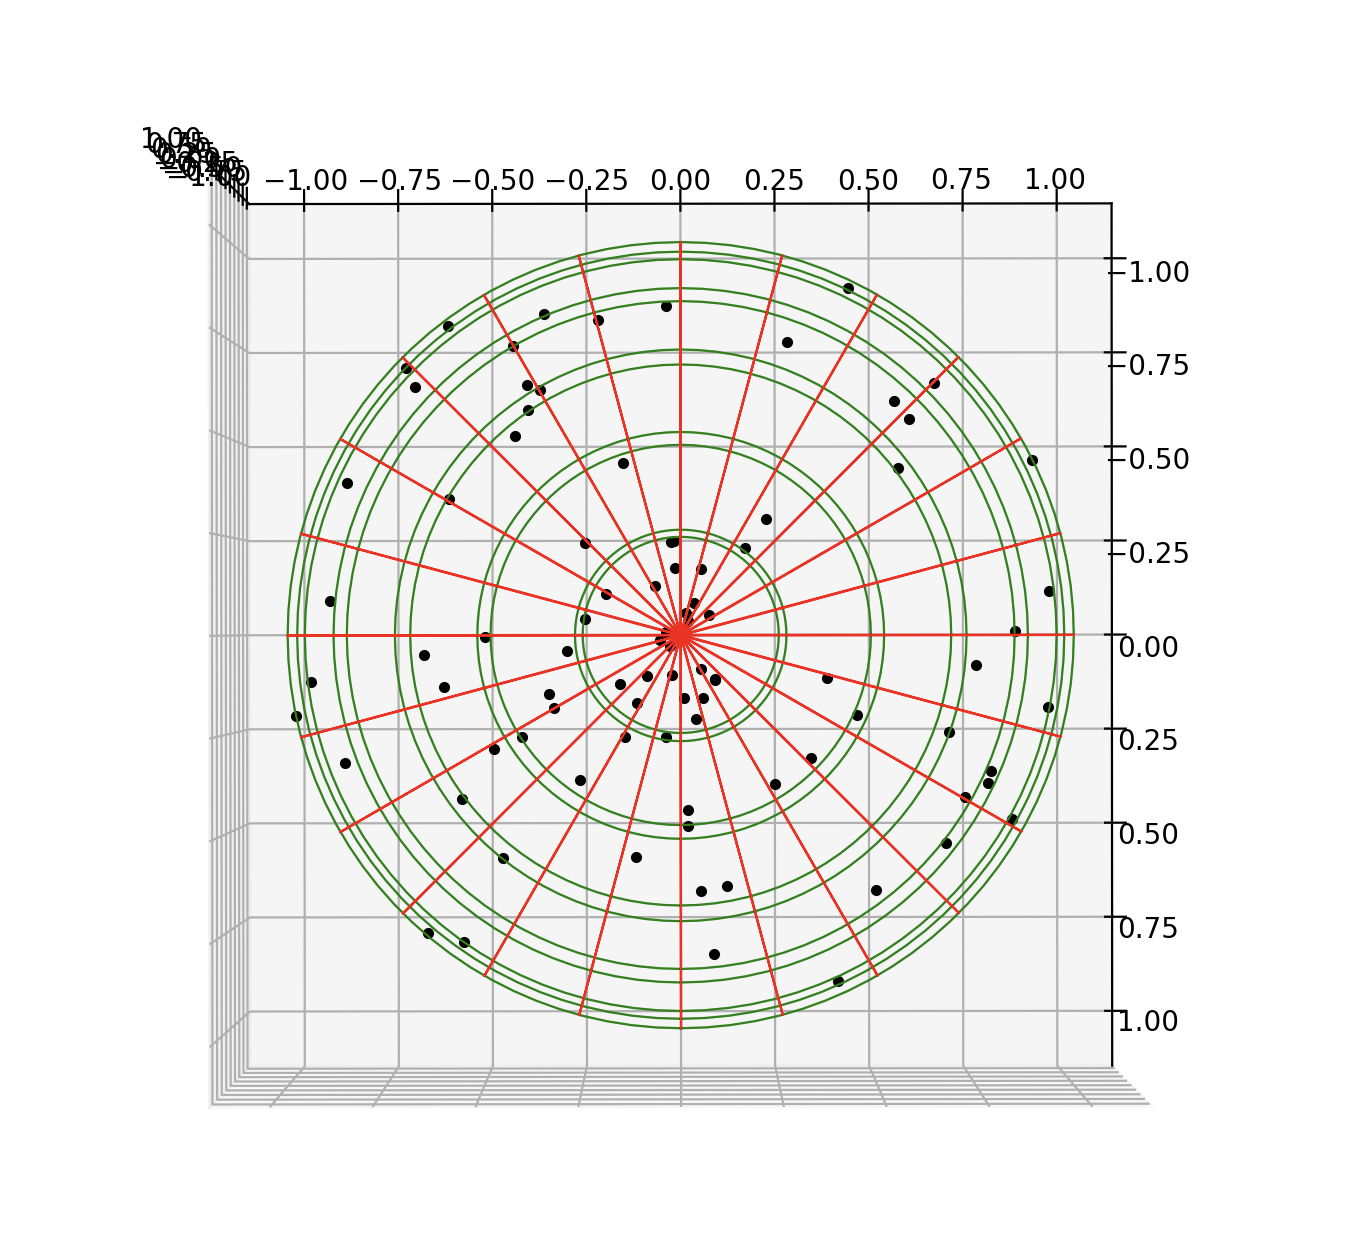
\includegraphics[width=1\linewidth]{SWIFT SGRB 3D.png}
    \caption{TOP VIEW}
  \end{subfigure}%
  \begin{subfigure}{.5\textwidth}
  \centering
    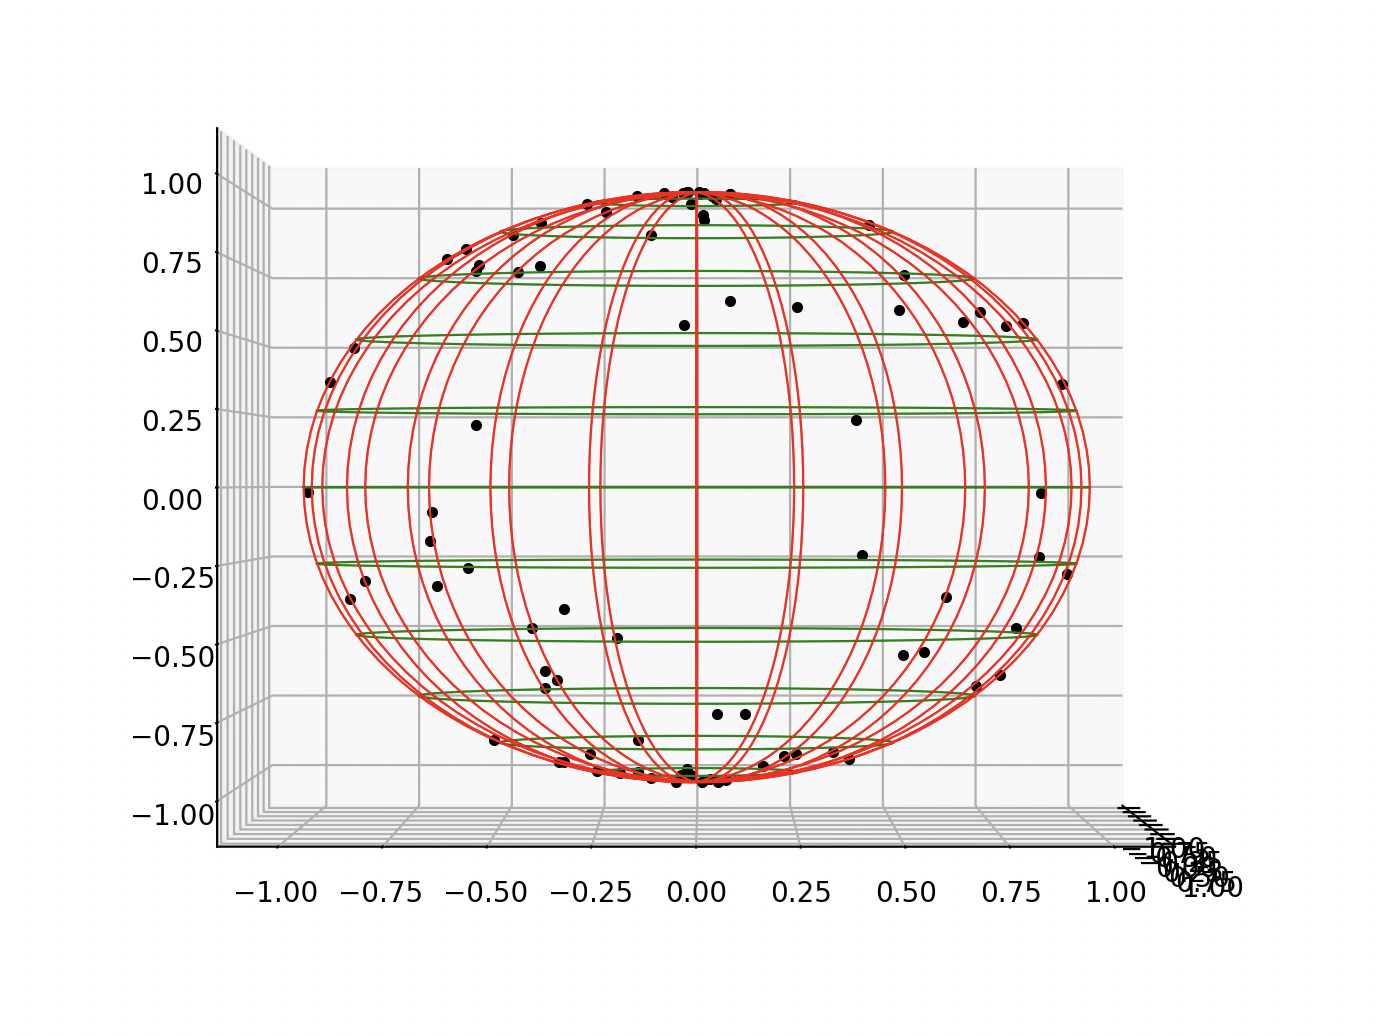
\includegraphics[width=1\linewidth]{SWIFT SGRB 3DD.png}
    \caption{SIDE VIEW}
  \end{subfigure}
  \caption{3D plot of the SWIFT SGRB sample. The results confirm it to be a homogeneous distribution.}
\end{figure}

\clearpage
\newpage
{\huge CHAPTER 4}
\section{1. RESULTS}


The GRB sub-sample with \(\sigma\)\textsubscript{­r­­} \textless{} 6° is
taken as our data set. Overall, we have 1242 GRBs from the SWIFT data set
( 1151 LGRBs and 92 SGRBs), 3612 GRBs from the FERMI data set ( 3016 LGRBs
and 596 SGRBs), and 1535 GRBs from the BATSE data set ( 1299 LGRBs and 236 SGRBs).

We can start by comparing the absolute sum tests with the corresponding 2pACF graphs. The shaded
region in the 2pACF graphs provide the allowed region in which the value
of the 2pACF for an intrinsic isotropic sample can vary due to
randomness. From these plots, we can conclude that both the 2pACF and
the absolute sum show a good agreement between the taken data sets and
the benchmark, and therefore no evidence against statistical isotropy.

We also show the result obtained from the non parametric tests (KS and
AD tests) in Table 1,2 and 3. We see that in most cases, the data set
passes the test and has a p value \textgreater{} 0.05, the exceptions
being FERMI SGRB, BATSE SGRB and the SWIFT LGRB datasets.


\section{2. DISCUSSION AND CONCLUSION}


The assumption of large-scale statistical homogeneity and isotropy is a
central idea in modern cosmology. These, along with
Einstein\textquotesingle s field equations, form the basis of modern
cosmology as we know it.

In this paper, we tested the statistical isotropy hypothesis of the
Cosmological principle by using the 2pACF of various GRB distributions.
We compared the 2pACF of isotropic synthetic sample with that of various
GRB datasets in order to carry out our research. In order to limit the
effect the positional uncertainties might have on our result, we
generated 100 MC realisations with new positions for the GRBs within
their observational position uncertainty. As large position
uncertainties may lead to specious drifts from isotropy, we perform cuts
on the positional uncertainty, choosing \(\sigma\)\textsubscript{­r­­} = 6°
as the cut-off. It is an optimum value as we avoid the spurious isotropy
while not losing too many sources. We then split the data into LGRB and
SGRB using the T­\textsubscript{90} value. We find that not all GRBs of
the data set have known T­\textsubscript{90} values and hence we lose
some sources here as well.

Overall, we did not find a good agreement between all these data and the
statistical isotropy hypothesis, since the 2pACF and the absolute sum
test does not agree with the benchmark simulations. This was also confirmed by
the two complementary KS and AD tests between the real data and the
benchmark, whose p-values are shown in Tables.

We remark that in the case of BATSE and FERMI SGRB, despite a lower
p-value, one still cannot reject the null hypothesis. In the case of
SWIFT and FERMI LGRB, the departure from isotropic behaviour might be due to some
other factor. Other studies which have also found statistical anisotropy
of LGRBs credit it to the impact of the sky exposure function. Our
departure from isotropy might also suggest that our testing was not
robust enough. Other studies take 1000+ Monte Carlo realisations, which
we aren't able to do here because such calculations will take a very
long amount of time on our computer hardware. Or it might just be that
this particular data set that we have taken is after all, anisotropic.

As the testing for isotropy has passed in most cases (by number of
GRBs), we conclude that there is no significant evidence for isotropy in the currently available GRB catalogues.
\newpage
{\huge CHAPTER 5}
\section{BIBLIOGRAPHY}
\printbibliography
\end{document}

